%%%%%%%%%%%%%%%%%%%%%%%%%%%%%%%%%%%%%%%%%
% Masters/Doctoral Thesis 
% LaTeX Template
% Version 2.5 (27/8/17)
%
% This template was downloaded from:
% http://www.LaTeXTemplates.com
%
% Version 2.x major modifications by:
% Vel (vel@latextemplates.com)
%
% This template is based on a template by:
% Steve Gunn (http://users.ecs.soton.ac.uk/srg/softwaretools/document/templates/)
% Sunil Patel (http://www.sunilpatel.co.uk/thesis-template/)
%
% Template license:
% CC BY-NC-SA 3.0 (http://creativecommons.org/licenses/by-nc-sa/3.0/)
%
%%%%%%%%%%%%%%%%%%%%%%%%%%%%%%%%%%%%%%%%%

%----------------------------------------------------------------------------------------
%	PACKAGES AND OTHER DOCUMENT CONFIGURATIONS
%----------------------------------------------------------------------------------------

\documentclass[
12pt, % The default document font size, options: 10pt, 11pt, 12pt
%oneside, % Two side (alternating margins) for binding by default, uncomment to switch to one side
english, % ngerman for German
onehalfspacing, % Single line spacing, alternatives: singlespacing, onehalfspacing or doublespacing
%draft, % Uncomment to enable draft mode (no pictures, no links, overfull hboxes indicated)
nolistspacing, % If the document is onehalfspacing or doublespacing, uncomment this to set spacing in lists to single
liststotoc, % Uncomment to add the list of figures/tables/etc to the table of contents
%toctotoc, % Uncomment to add the main table of contents to the table of contents
parskip, % Uncomment to add space between paragraphs
%nohyperref, % Uncomment to not load the hyperref package
headsepline, % Uncomment to get a line under the header
%chapterinoneline, % Uncomment to place the chapter title next to the number on one line
consistentlayout, % Uncomment to change the layout of the declaration, abstract and acknowledgements pages to match the default layout
]{MastersDoctoralThesis} % The class file specifying the document structure

\usepackage[utf8]{inputenc} % Required for inputting international characters
\usepackage[T1]{fontenc} % Output font encoding for international characters

\usepackage{mathpazo} % Use the Palatino font by default
\usepackage{color}
\usepackage{subfigure}
\usepackage{array}
\usepackage{listings}
\usepackage{amssymb}
\usepackage{ifthen}
\usepackage{float}
\usepackage{lscape}
\newcolumntype{C}[1]{>{\centering\let\newline\\\arraybackslash\hspace{0pt}}m{#1}}
\newcolumntype{L}[1]{>{\centering\let\newline\\\arraybackslash\hspace{0pt}}p{#1}}
\usepackage{hyperref}
\lstset{numbers=left, basicstyle=\footnotesize, frame=single, breaklines=true, breakatwhitespace=true}

\usepackage[backend=bibtex]{biblatex} % Use the bibtex backend with the authoryear citation style (which resembles APA)

\addbibresource{example.bib} % The filename of the bibliography

\usepackage[autostyle=true]{csquotes} % Required to generate language-dependent quotes in the bibliography

\newcommand{\projectName}{\textbf{ProjectName} }

%----------------------------------------------------------------------------------------
%	MARGIN SETTINGS
%----------------------------------------------------------------------------------------

\geometry{
	paper=a4paper, % Change to letterpaper for US letter
	inner=2.5cm, % Inner margin
	outer=3cm, % Outer margin
	bindingoffset=.5cm, % Binding offset
	top=1.5cm, % Top margin
	bottom=1.5cm, % Bottom margin
	%showframe, % Uncomment to show how the type block is set on the page
}

%----------------------------------------------------------------------------------------
%	THESIS INFORMATION
%----------------------------------------------------------------------------------------

\thesistitle{Automatic Visual Regression Testing using container orchestration for Web Apps running on Chromium and Webkit} % Your thesis title, this is used in the title and abstract, print it elsewhere with \ttitle
\supervisor{Mario \textsc{Linares-Vásquez}} % Your supervisor's name, this is used in the title page, print it elsewhere with \supname
\examiner{} % Your examiner's name, this is not currently used anywhere in the template, print it elsewhere with \examname
\degree{Systems and Computation Engineering} % Your degree name, this is used in the title page and abstract, print it elsewhere with \degreename
\authorone{Sergio \textsc{Guzmán-Mayorga}} % Your name, this is used in the title page and abstract, print it elsewhere with \authoronename
\authortwo{Julián \textsc{Alberto-Manrique}} % Your name, this is used in the title page and abstract, print it elsewhere with \authoronename
\addresses{} % Your address, this is not currently used anywhere in the template, print it elsewhere with \addressname

\subject{Biological Sciences} % Your subject area, this is not currently used anywhere in the template, print it elsewhere with \subjectname
\keywords{} % Keywords for your thesis, this is not currently used anywhere in the template, print it elsewhere with \keywordnames
\university{\href{http://uniandes.edu.co}{Universidad de los Andes}} % Your university's name and URL, this is used in the title page and abstract, print it elsewhere with \univname
\department{\href{http://sistemas.uniandes.edu.co}{Systems and Computing Engineering Department}} % Your department's name and URL, this is used in the title page and abstract, print it elsewhere with \deptname
\group{\href{https://ticsw.uniandes.edu.co/}{TICSw research group}} % Your research group's name and URL, this is used in the title page, print it elsewhere with \groupname
\faculty{Faculty of Engineering} % Your faculty's name and URL, this is used in the title page and abstract, print it elsewhere with \facname

\AtBeginDocument{
\hypersetup{pdftitle=\ttitle} % Set the PDF's title to your title
\hypersetup{pdfauthor=\authoronename-\authortwoname} % Set the PDF's author to your name
\hypersetup{pdfkeywords=\keywordnames} % Set the PDF's keywords to your keywords
}
\newcommand\SANTIAGO[1]{\textcolor{red}{\nb{SANTIAGO}{#1}}}


\definecolor{orange}{rgb}{1,0.5,0}

\makeatletter

% this  is a easy way to add and highlight new text  ...
% just comment in/out the \tnew macro ..

\newcommand{\tnew}[1]{{\bf { #1 }} }
%\newcommand{\tnew}[1]{{ { #1 }} }

% math and theorem definition

\newcommand{\ndef}{\stackrel{\rm def}{=}}

% this is used for draft only

%\renewcommand{\baselinestretch}{2}

% just to number pages in the draft

\pagenumbering{arabic}

% nothing i.e., no-numbering final and camera ready

%\pagestyle{empty}


\newboolean{showcomments}


\setboolean{showcomments}{true}

\ifthenelse{\boolean{showcomments}}
  {\newcommand{\nb}[2]{
    \fbox{\bfseries\sffamily\scriptsize#1}
    {\sf\small$\blacktriangleright$\textit{#2}$\blacktriangleleft$}
   }
   \newcommand{\cvsversion}{\emph{\scriptsize$-$Id: macro.tex,v 1.9 2005/12/09 22:38:33 giulio Exp $}}
  }
  {\newcommand{\nb}[2]{}
   \newcommand{\cvsversion}{}
  }



\newcommand\CAMILOO[1]{\textcolor{red}{\nb{CAMILO}{#1}}}
\newcommand\CAMILO[1]{\textcolor{orange}{\nb{CAMILO}{#1}}}

\newcommand\MARIO[1]{\textcolor{red}{\nb{MARIO}{#1}}}

\newcommand{\cmark}{\ding{51} }%
\newcommand{\xmark}{\ding{55}}%
\newcommand\fix[1]{\textbf{FIX THIS}{#1}}
\newcommand{\here}{\textcolor{red}{\textbf{***}{CONTINUE HERE}}}
\newcommand{\ie}{\textit{i.e.,}\xspace}
\newcommand{\eg}{\textit{e.g.,}\xspace}
\newcommand{\etc}{\textit{etc.}\xspace}
\newcommand{\etal}{\textit{et al.}\xspace}
\newcommand{\libra}{{\sc Libra}\xspace}
\newcommand{\secref}[1]{Section~\ref{#1}\xspace}
\newcommand{\chapref}[1]{Chapter~\ref{#1}\xspace}
\newcommand{\appref}[1]{Appendix~\ref{#1}\xspace}
\newcommand{\figref}[1]{Fig.~\ref{#1}\xspace}
\newcommand{\listref}[1]{Listing~\ref{#1}\xspace}
\newcommand{\tabref}[1]{Table~\ref{#1}\xspace}
\newcommand{\sotag}[1]{<#1>\xspace}
\newcommand{\todoref}{\textcolor{red}{[REF]}}
\newcommand{\tool}{\texttt{MutAPK} \xspace}




\begin{document}

\frontmatter % Use roman page numbering style (i, ii, iii, iv...) for the pre-content pages

\pagestyle{plain} % Default to the plain heading style until the thesis style is called for the body content

%----------------------------------------------------------------------------------------
%	TITLE PAGE
%----------------------------------------------------------------------------------------

\begin{titlepage}
\begin{center}


% {\scshape\LARGE \univname\par}\vspace{1.5cm} % University name
\begin{figure}[h]
\centering

\includegraphics[width=0.4\textwidth]{../Figures/logoUniandes}
\end{figure}
%\vspace*{.07\textheight}
%\textsc{\Large Master Thesis}\\
\vspace{0.3cm} % Thesis type

\HRule \\[0.4cm] % Horizontal line
{\huge  \ttitle\par}\vspace{0.4cm} % Thesis title
\HRule \\[1cm] % Horizontal line
 
\begin{minipage}[t]{0.4\textwidth}
\begin{flushleft} \large
\emph{Authors:}\\
\href{http://sguzmanm.github.io}{\authoronename{}} % Author name - remove the \href bracket to remove the link
\href{http://sxubas.github.io}{\authortwoname{}} % Author name - remove the \href bracket to remove the link
\end{flushleft}
\end{minipage}
\begin{minipage}[t]{0.3\textwidth}
\begin{flushright} \large
\emph{Advisor:} \\
\href{https://profesores.virtual.uniandes.edu.co/mlinaresv/en/inicio-en/}{\supname} % Supervisor name - remove the \href bracket to remove the link  
\end{flushright}
\end{minipage}\\[1.5cm]
 
\vfill

\large \textit{A thesis submitted in fulfillment of the requirements\\ for the degree of \degreename}\\%[0.1cm] % University requirement text
\textit{in}\\%[0.3cm]
%\groupname
\begin{figure}[h]
\centering

\includegraphics[width=0.5\textwidth]{../Figures/tsdlLargo}
\end{figure}
\deptname\\[0.5cm] % Research group name and department name
 
\vfill

{\large \today}\\
%[4cm] % Date
%\includegraphics{F} % University/department logo - uncomment to place it
 
\vfill
\end{center}
\end{titlepage}

%----------------------------------------------------------------------------------------
%	QUOTATION PAGE
%----------------------------------------------------------------------------------------

\vspace*{0.2\textheight}

\noindent\enquote{\itshape You can't connect the dots looking forward; you can only connect them looking backwards. So you have to trust that the dots will somehow connect in your future. You have to trust in something - your gut, destiny, life, karma, whatever.}\bigbreak

\hfill Steve Jobs

%----------------------------------------------------------------------------------------
%	ABSTRACT PAGE
%----------------------------------------------------------------------------------------

\begin{abstract}
\addchaptertocentry{\abstractname} % Add the abstract to the table of contents
TODO: Fill with summary for the whole thesis
\end{abstract}

%----------------------------------------------------------------------------------------
%	ACKNOWLEDGEMENTS
%----------------------------------------------------------------------------------------

%\begin{acknowledgements}
%\addchaptertocentry{\acknowledgementname} % Add the acknowledgements to the table of contents
%To Google for helping me get a PhD position :D
%\end{acknowledgements}


%----------------------------------------------------------------------------------------
%	LIST OF CONTENTS/FIGURES/TABLES PAGES
%----------------------------------------------------------------------------------------

\tableofcontents % Prints the main table of contents

\listoffigures % Prints the list of figures

\listoftables % Prints the list of tables

%----------------------------------------------------------------------------------------
%	ABBREVIATIONS
%----------------------------------------------------------------------------------------

%\begin{abbreviations}{ll} % Include a list of abbreviations (a table of two columns)

%\textbf{APK} & \textbf{A}ndroid A\textbf{p}plication Pac\textbf{k}age\\

%\end{abbreviations}

%----------------------------------------------------------------------------------------
%	SYMBOLS
%----------------------------------------------------------------------------------------

%\begin{symbols}{lll} % Include a list of Symbols (a three column table)

%$a$ & distance & \si{\meter} \\
%$P$ & power & \si{\watt} (\si{\joule\per\second}) \\
%Symbol & Name & Unit \\

%\addlinespace % Gap to separate the Roman symbols from the Greek

%$\omega$ & angular frequency & \si{\radian} \\

%\end{symbols}

%----------------------------------------------------------------------------------------
%	DEDICATION
%----------------------------------------------------------------------------------------

%\dedicatory{For/Dedicated to/To my\ldots} 

%----------------------------------------------------------------------------------------
%	THESIS CONTENT - CHAPTERS
%----------------------------------------------------------------------------------------

\mainmatter % Begin numeric (1,2,3...) page numbering

\pagestyle{thesis} % Return the page headers back to the "thesis" style

% Include the chapters of the thesis as separate files from the Chapters folder
% Uncomment the lines as you write the chapters

% Chapter Template

\chapter{Introduction} % Main chapter title

\label{Chapter1} % Change X to a consecutive number; for referencing this chapter elsewhere, use \ref{ChapterX}

TODO: Do the intro for the project once it is fulfilled

Mobile markets have pushed and promoted the raising of an interesting phenomenon that has permeated not only developers culture, but also human beings’ daily life activities. Mobile devices, apps, and services are helping companies and organizations to make “digital transformation” possible through services and capabilities that are offered ubiquitously and closer to the users. Nowadays, mobile apps and devices are the most common way for accessing those services and capabilities; in addition, apps and devices are indispensable tools for allowing humans to have in their phones, computational capabilities that make life better and easier.

The mobile apps phenomenon has also changed drastically the way how practitioners design, code, and test apps.  Mobile developers and testers face critical challenges on their daily life activities such as (i) continuous pressure from the market for frequent releases of high quality apps, (ii) platform fragmentation at device and OS levels, (iii) rapid platform/library evolution and API instability, and (iv) an evolving market with millions of apps available for being downloaded by ends users \cite{joorabchi2013real,palomba2018crowdsourcing}. Tight release schedules, limited developer and hardware resources, and cross-platform delivery of apps, are common scenarios when developing mobile apps \cite{joorabchi2013real}. Therefore, reducing the time and effort devoted to software engineering tasks while producing high quality mobile software is a ``precious’’ goal.

Both practitioners and researchers, have contributed to achieve that goal, by proposing approaches, mechanisms, best practices, and tools that make the development process more agile. For instance, cross-platform languages and frameworks (e.g., Flutter, Ionic, Xamarin, React Native) contribute to reducing the development time by providing developers with a mechanism for building Android and iOS versions of apps in a write-one-run-anywhere way \cite{joorabchi2013real,fazzini2017automated}. Automated testing approaches help testers to increase the apps' quality and reduce the detection/reporting time \cite{choudhary2015automated,kochhar2015understanding,linares2017continuous}. 
Automated categorization of reviews also helps developers to select relevant information, issues, features and sentiments, from large volume of review that are posted by users \cite{palomba2018crowdsourcing,villarroel2016release,di2016would}. Moreover, approaches for static analysis, are helping developers to early detect different types of bugs and issues that without the automated support could be time consuming for developers --- when doing the analysis manually \cite{li:IST2017}. 
Both static and dynamic analyses have been used with the aforementioned approaches, with a special preference for static analysis on source code.  

The developers community is quickly moving towards using cloud-services and crowd-sourced services for software engineering tasks \cite{Leicht2017IEEESoftware, stol2017crowdsourcing}; using those services is becoming a common practice of mobile developers who want to reduce costs and the time devoted for an activity. For example, the Firebase Test Lab platform \cite{firebase} provides automated testing services, in particular, it automatically executes/explores a given app (provided by the developer as an Android APK file), and reports crashes found on a devices matrix that is selected by the user. However, the lack of knowledge of source code internals imposes a limitation on the usefulness and completeness of the results reported back to the users.

%----------------------------------------------------------------------------------------
%	SECTION 1
%----------------------------------------------------------------------------------------

\section{Problem Statement}

The power and usefulness of a large number of  state-of-the-art approaches for automated software engineering of Android apps rely on the existence of source code for extracting intermediate representations or models that drive the analysis execution or the artifacts generation. For example, Zaeem \textit{et al.}\cite{zaeem2014automated} instrumentates the source code in order to record the view flow followed through a set of instructions in order to validate oracles. However, existing approaches that rely on source code for supporting automated software engineering tasks are untenable in a commercial environment where practitioners  outsource software engineering tasks, but without releasing the source code (i.e., the services work directly on executable files). 

Any type of analysis that relies only on executable files (i.e., dynamic analysis) is known to be limited when compared to static analysis that can be done directly on the code \cite{spathoulas2014assessing}. For example, Firebase Test Lab enables automated tests based on Random GUI input generation. However, this test provides low usage case coverage. Additionally, for different legal and organizational reasons (e.g., source code contains a company's exclusive implementation of an algorithm, source code contains keys/secrets for services, etc.) the app's source code is often not available, making it difficult to enable cloud/crowd-based services that use state-of-the-art approaches.

Furthermore, as it will be shown in the Section 2, decompilation/compilation process is a cumbersome process due to the wide spectrum of developing possibilities that defines how each application is build. Software Engineering approaches that rely on source code modifications/instrumentation, and then require to build/compile the app are expensive; as is the case of mutation testing \cite{appelt2014automated,linares2017enabling,praphamontripong2016experimental,rodriguez2018mutode}.

\section{Thesis  Goals}

Consequently, the goal of this thesis is to \emph{enable automated software engineering (ASE) tasks for Android apps, at APK level (i.e., using intermediate representations instead of source code)}. With this, ASE tasks can be crowd-sourced and delegated to third party services without having to release applications source code. In the particular case of this thesis, we focused on mutation testing. 

In particular, the specific objectives of this master thesis are:
\begin{itemize}
	\item Propose a novel framework aimed at enabling automated software engineering tasks for Android apps
	at APK level (\textit{i.e.,} without the need of source code).
	\item Validate the feasibility of our proposed approach through implementing it for mutation testing.
	\item Evaluate the performance of the proposed approach for mutation testing at APK level, when compared to a state-of-the-art tool for mutation testing at source code level.
\end{itemize}

\section{Thesis contribution}

As a complement to the existent approaches for analysis of APKs, we propose a way for enabling automated software engineering tasks for closed-source Android apps, and in particular, by working at the level of APK files (i.e., android executable packages), similarly to the way how practitioners use third-party services (i.e., delivering only executable files). To this, our primary goal is to automatically extract models directly from APK files and without decompiling the package to the original source code, which is time consuming, prone to decompilation/compilation errors, and could reveal private artifacts included into the code. Then, our second goal is to implement  approaches for automated software engineering tasks on the models extracted from the APKs.

As an initial step and representative example in a long term research agenda, we enabled mutation testing at APK level, by (i) translating the 38 mutant operation rules defined by Linares-Vásquez \textit{et. al.}\cite{linares2017enabling}, (ii) implementing 35 mutation operators for mobile apps using SMALI representation that leads to compilable/installable applications, and (iii) evaluating whether the approach improves generation and building times when compared to a mutation testing tool that works with original source code. The results from our empirical study shows that extracting the models from APK files is feasible without implementing decompilation pipelines that recover the original source code. 

\begin{table}[!ht]
	\centering
	\caption{Summary of results when comparing  MutAPK and MDroid+. *Efectivity Rate is measured as the percentage of the total time that correspond to the compiled mutants }
	\label{tab:bcmamdp}
	\begin{tabular}{|L{4cm}|c|c|}
		\hline
		Metric Name&MutAPK&MDroid+\\
		\hline \hline
		Amount of Mutants Generated & 74256 & 8847 \\ \hline
		Average Mutation Time&144.66ms&4.61s\\ \hline
		Amount of Compiled Mutants&72362&8797\\ \hline
		Average Compilation Time &12.42s&3.25min\\ \hline
		Average Complete Mutant Creation Time & 12.56s& 3.33min\\ \hline
		Efectivity Rate* & 97,44\%&99,43\%\\
		\hline
	\end{tabular}
\end{table}

Our initial results suggest that in terms of creation/building time and number of mutants, modifying APKs directly outperforms mutants generation at source code level. As it can be seen in Table \ref{tab:bcmamdp}, MutAPK compared with MDroid+\footnote{Data collected from MDroid+ FSE/ESEC replication package. \url{https://www.android-dev-tools.com/s/FSE-Online_Appendix-Data.zip}}, generates 13 times more mutants, reduces (on average)  the time to mutate a copy of the app in a ~96\%, generates 7 times more compiled mutants, and reduces  the time required to compile a mutant in a ~93\%, when compared to MDroid+. However, there is room for improvement in the mutants implementation because there are mutants that generate compilations errors, and its non-compilable mutants rate is larger than MDroid+'s.

Therefore, from the previously presented result we can say that MutAPK improves the state of the mutation testing environment using the 6.36\% of the time (required by MDroid+) to generate 13 times more mutants. At the same time, due to the improvement on the mutant creation time (\textit{i.e.,} mutant generation + mutant compilation), MutAPK also increases the available time that users can invest in running theirs test suites over the mutants; moreover, due to the improvement in the number of generated mutants, we might generate a more comprehensive representation of the search space of possible errors a mobile application can have.


As part of the process followed in this thesis we published four issues in the MDroid+ repository and interacted with MDroid+ maintainers. We fixed three of the open issues.

Finally, MutAPK as tool is the first one that performs Mutation Testing for Android Apps at APK level. MutAPK can be downloaded from its public repository \cite{MutAPK}.


\section{Document Structure}
This document is organized as follows: in Chapter 2 we describe some concepts that will help the reader to understand the context of the thesis. Chapter 3 presents the previous work done in terms of Static analysis of Android Apps and Mutation Testing for Android Apps. Chapter 4 explains the proposed novel framework and its implementation using Mutation Testing, along with an explanation of MutAPK functioning. Chapter 5 presents the study designed and performed to understand the impact of generating mutants at APK level by 5 metrics defined around mutant generation. Chapter 6 present the conclusions of our research work and Chapter 7 shows the future work for this research.



% Chapter Template

\chapter{Context} % Main chapter title

\label{Chapter2} % Change X to a consecutive number; for referencing this chapter elsewhere, use \ref{ChapterX}

%----------------------------------------------------------------------------------------
%	SECTION 1
%----------------------------------------------------------------------------------------

\section{Mutation Testing}

Mutation testing is a testing technique which consists on modifying an application (by injecting bugs) in order to enhance and evaluate the quality of the test suite that accompanies it. Each injected bug generates a new version of the application, and its called \textbf{mutant}. Each mutant differs from the original version in a simple modification, called \textbf{mutation}. As an example, if there is a compound logical operation in the original version, a valid mutation consists in replacing one and only one of the logical operators in the compound operation (i.e. if there is an "AND", the mutation changes  it with "OR"). It is worth noticing, that the replacement of each operator in the compound operation generates one mutant.

Now, to determine how many mutants can be generated, mutation testing uses a set of rules called \textbf{mutation operators} that define common errors and practices that belong to programming rules (e.g., replace a math operator ), or to the specific programming language context (e.g., assign a null value to an Intent parameter ). Therefore, depending on the tool used to generate the mutants, the application to be mutated is analyzed to derive a Potential Fault Profile \cite{linares2017enabling,Moran:ICSE18}, i.e., a set of possible locations where a mutant operator can be applied. For each of this locations the mutation tool creates a copy of the original app, and this copy is a modification produced by applying a mutation operator. Several mutation operators have been proposed for different types of applications such as web apps \cite{praphamontripong2016experimental}, data-centric apps \cite{appelt2014automated}, NodeJS packages \cite{rodriguez2018mutode} and Android apps \cite{linares2017enabling}. Table \ref{table:mtpfsc} summarizes different implementations of mutation testing in several programming languages and for different types of applications.

For more information about mutation testing you can refer to Chapter 5 of Paul Ammann and Jeff Offutt book called Introduction to Software Testing \cite{ammann2016introduction}, or the survey by Jia and Harman \cite{Jia:TSE11}.

\begin{table}[H]
	\centering
		\caption{Mutation testing papers for different application types.}
	\label{table:mtpfsc}
	\begin{tabular}{|p{3cm} | p{10cm}|} 
		\hline
		App type/Language & Paper \\ [0.5ex] 
		\hline\hline
		Java & Yu-Seung Ma, Yong Rae Kwon, and Jeff  Offutt. 2002. \textbf{\textit{Inter-Class Mutation Operators for Java.}} In 13th International Symposium on Software Reliability Engineering (ISSRE’02) \\
		\hline\hline
		Python & Anna Derezinska and Konrad Halas. 2014. \textbf{\textit{Analysis of Mutation Operators for the Python Language.}} Proceedings of the Ninth International Conference on Dependability and Complex Systems (DepCoS14) \\ \hline\hline
		Web Apps & Upsorn Praphamontripong, Je  Outt, Lin Deng, and Jingjing Gu. \textbf{\textit{An Experimental Evaluation of Web Mutation.}} ICSTW’16 \\ \hline\hline
		Data-Centric Apps & Dennis Appelt, Cu Duy Nguyen, Lionel C. Briand, and Nadia Alshahwan.\textit{ \textbf{Automated testing for SQL injection vulnerabilities: an input mutation approach.}} ISSTA’14 \\ \hline\hline
		GUIS & R. A. P. Oliveira, E. Alégroth, Z. Gao, and A. Memon. \textbf{\textit{Definition and evaluation of mutation operators for GUI-level mutation analysis.}} ICSTW’15 \\ \hline\hline
		Test Data & Daniel Di Nardo, Fabrizio Pastore, and Lionel C. Briand. 2015. \textbf{\textit{Generating Complex and Faulty Test Data through Model-Based Mutation Analysis.}} ICST’15 \\
		\hline\hline
		Android & Mario Linares-Vásquez, Gabriele Bavota, Michele Tufano, Kevin Moran, Massimiliano Di Penta, Christopher Vendome, Carlos Bernal-Cárdenas and Denys Poshyvanyk. 2017. \textit{\textbf{Enabling Mutation Testing for Android Apps}}. ESEC/FSE 2017 \\
		\hline\hline
		NodeJS & Diego Rodríguez-Baquero, and Mario Linares-Vásquez. 2018. \textit{\textbf{Mutode: generic JavaScript and Node. js mutation testing tool}}. ISSTA 2018 \\
		\hline
	\end{tabular}
\end{table}


\section{Android App Building Process}

In order to understand some of the problems and design decisions  in this thesis, it is important to know how android applications are built from the source code into an Android Application Package ( APK ), which is the file deployed to an Android device. It is worth noticing that Android applications can be developed in several ways, whether using first-class languages\footnote{text} as JAVA, Dart or Kotlin, or using frameworks for cross-platform development (e.g. Ionic, Phonegap, React4Native). Nevertheless, native approaches generates a project in a first-class language to be deployed in mobile devices. Therefore, for the purpose of this explanation lets assume the application to study was developed using a first-class (i.e., native) language. 

Resource files (i.e., color.xml, strings.xml, etc.), application files (e.g, *.java) , libraries  (i.e, jar files) and the Android manifest file are packaged in an APK file. The process starts with compiling the app source code to java bytecode, and then compiling bytecode  and libraries to dex code. Dex code is the set of operations that are going to be executed by the VM in an Android device. Previously generated files along with the already compiled libraries are compiled using the  \textit{dx} tool into one or several .dex files\footnote{For more information about multidex visit: \url{https://developer.android.com/studio/build/multidex?hl=es-419}}. Finally, packaged resource files and dex file(s) are packaged into an unsigned apk. So, while Java, Kotlin and Dart are high-level languages, dex operates as an intermediate representation that is closer to the machine.

\begin{figure}[h!]
	\caption{Android Building process.}
	\centering
	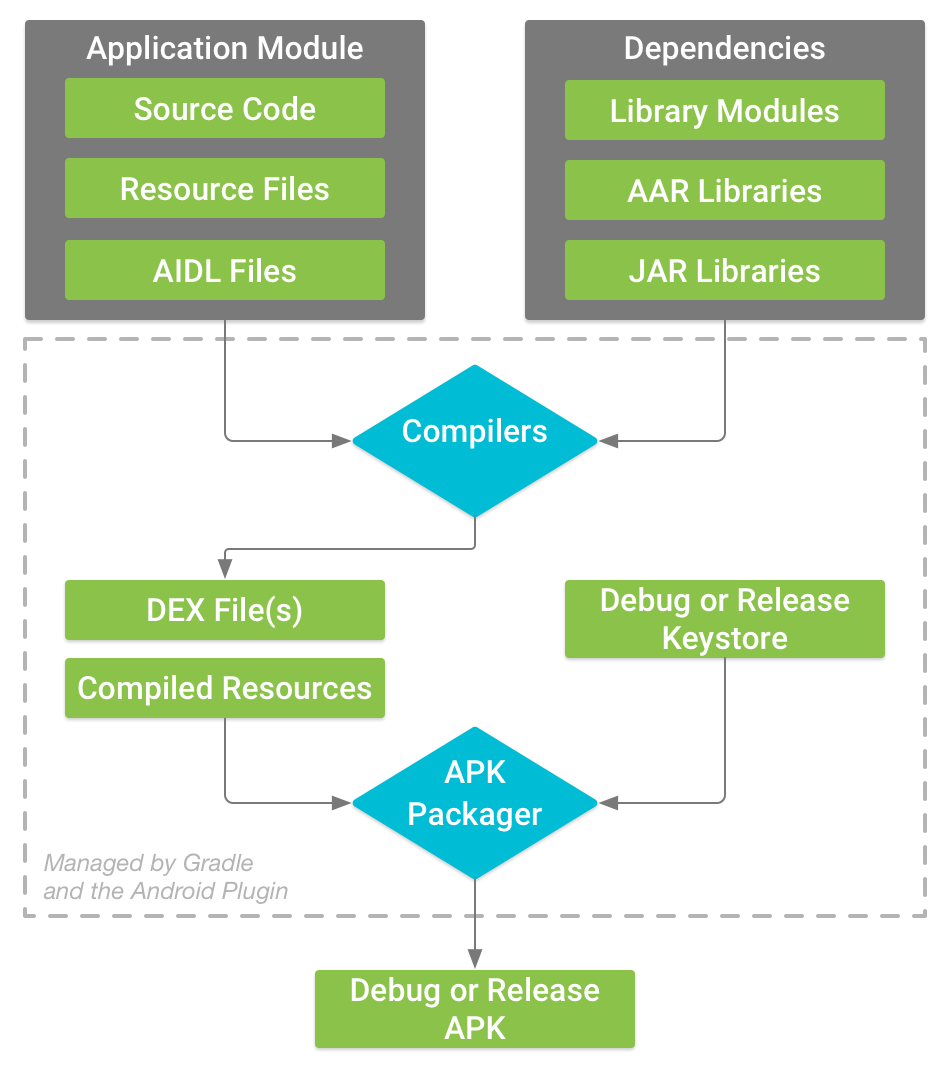
\includegraphics[width=0.7\textwidth]{../Figures/android-build-process.png}
	\label{fig:abp}
\end{figure}


\section{Intermediate Representations (IR)}

An intermediate representation is a representation of the source code aimed at being more expressive  and easier of interpretation for a machine. An intermediate representation has the property that without losing app behavior, it presents the source code in a less complex format or in a less cumbersome context, from the point of view of a machine. In the specific case of Android apps, there are several intermediate  representation; we will briefly describe 4  of the them, that have been widely used in research.:  Java Bytecode, Dex, Smali, and Jimple. The first two are the closer representations to the starting and ending point of the Android application building process, while the other two (even being closer to the endpoint) have been created with the purpose of enabling analysis tasks on the source code. 

One of the benefits of using intermediate representations (in the context of JAR and APK analysis) is avoiding the decompilation of the app to reach the original source code; in the specific case of Android apps, by using an intermediate representation we get rid of reversing the android building process.

\subsection{JAVA Bytecode}

This intermediate representation is used by the Java Virtual Machine (JVM). It is worth noting that JVM follows a stack-based architecture \cite{jvms}. The most common way to get into this representation is through JAVA itself. However, there are compilers for other languages and frameworks into Java Bytecode. For example, SCALA, Clojure, Object Pascal, Kotlin and others \cite{pljvm}. As presented previously, Java Bytecode is the first resulting representation when compiling an android application source code.

\subsection{Dalvik Bytecode (DEX)}

Originally designed to work with Dalvik VM (DVM) and the Android Runtime (ART), the dalvik bytecode was designed for systems as mobile devices that have restrictions in their computational power \cite{dvmi, jitcadvm}. Actually, the Dalvik VM has been replaced by the Android Runtime (ART) keeping the same dalvik bytecode as representation to its execution. It is worth noting  that both DVM and ART follow a register-based architecture that normally requires fewer, but typically more complex VM instructions.

\subsection{JIMPLE}

Jimple is an intermediate representation used by Soot \cite{soot}. Jimple is based in 15 different operations that compared with the over 200 operations defined for Java bytecode makes it easier to optimize, however a lot of information can be lost when translated from java bytecode to Jimple.

\subsection{SMALI}

SMALI is an intermediate representation created by Ben Gruver \cite{smali}. It offers a readable version of the Dalvik bytecode, due to the similar amount of operations supported for both representations. As it is closer to dalvik bytecode rather than Java bytecode it represent the code following a register-based architecture. This enhances our possibilities to analyze applications because all Java instructions tend to be separated from recursive calls. For example, if a new object is created inside the parameter field of a method, SMALI translates the object creation into one line and the method call into another as it can be seen in Figure \ref{fig:sre}. Because of this, as it will be seen in next sections, we were able to recognize more potential fault injection points that are more complex to be recognized when analyzed in Java.

\begin{figure}[H]
	\caption{SMALI representation example}
	\centering
	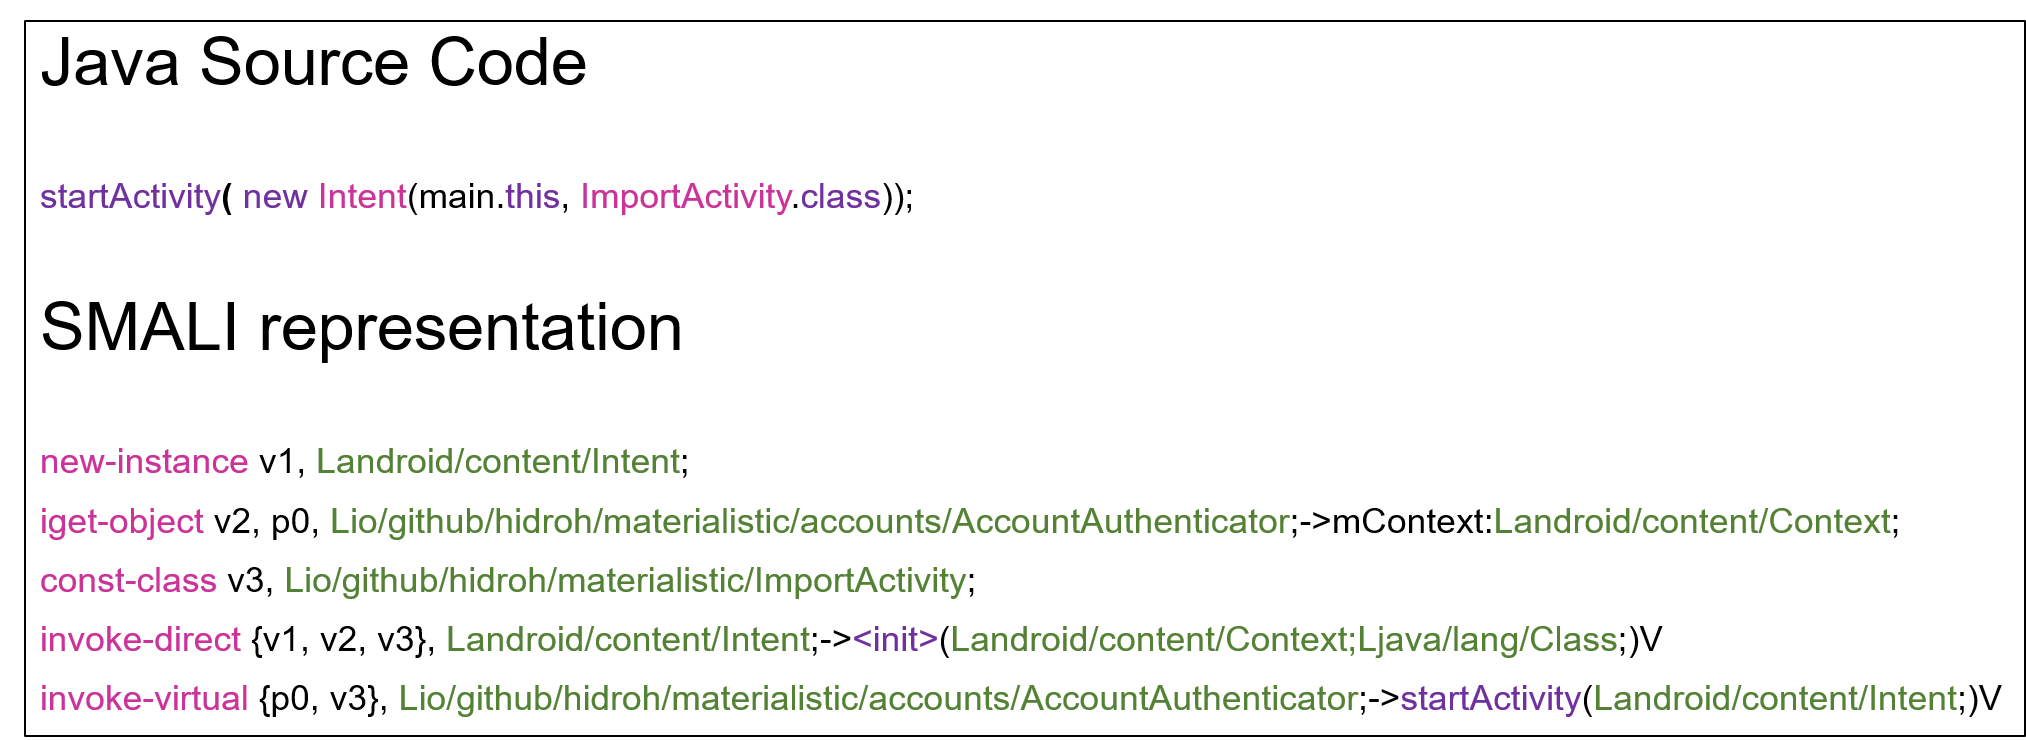
\includegraphics[width=\textwidth]{../Figures/smali}
	\label{fig:sre}
\end{figure}



% Chapter Template

\chapter{Related work} % Main chapter title


\label{ChapterX} % Change X to a consecutive number; for referencing this chapter elsewhere, use \ref{ChapterX}

The state of the art related to this particular project is classified on four different types of solutions that focus on giving developers tools to test their web applications on different kinds of platforms: Proprietary solutions, crowd sourced testing, open source software and scientific research.

%----------------------------------------------------------------------------------------
%	SECTION 1
%----------------------------------------------------------------------------------------

\section{Proprietary Solutions}

This is a niche of solutions for testing fragmentation on web applications: BrowserStack, SouceLabs, LambdaTest, Browserling, CrossBrowserTesting, just to name a few. Coming up, we will expose some of them that offer a free trial to test what they can offer.

\subsection{BrowserStack}
TODO: Fill out with content from proposal

\subsection{LambdaTest}
TODO: Fill out with content from proposal

\section{Crowd sourced testing}
Crowd sourced testing consists on distributing an application for testing on different machines and pay those who are willing to execute tests for such software. Although it is common in other types of software like games and mobile apps, it is not viable for web, since it requires a high costs compared to automation tools. 
Besides, it does not have the possibility to scale so easily as automated tests do. Meaning, one round of crowd sourced testing covers a specific version of the software; in order to test another version with corrections, other round is required, which is time and money consuming. Since web applications change constantly, this option becomes non-practical on the real life. 

\section{Open Source Software}

\subsection{Galen}

TODO: Fill out with information

\subsection{BackstopJS}

TODO: Fill out with information

\section{Scientific Research}

Taking a look into the literature, there are two main methods that offer developers the opportunity to know how their application looks in different browsers: Visual regression testing and runtime code analysis. 

\subsection{Visual regression testing}

It consists in generating images that show the places or actions where the same application is different when compared to a different browser. Alongside this line of research you can find tools like WEBDIFF and CrossCheck.

\textbf{WEBDIFF.} The main idea is to collect information from the DOM of each browser and capture a screenshot of the web page at a given time. Then. having a reference browser, mark all elements that vary when compared to such DOM. Finally, compare the information using the images and generate a list of elements that are different. 

\textbf{CrossCheck.} Use of the best of two different tools: Webdiff (Already explained above) and CROSST. Meanwhile Webdiff is very useful for detecting XBIs related to how the screen looks in different browsers, CROSST is used for finding trace-level XBIs. When talking about trace-level, we refer to detection of differences on the elements of the DOM by performing a static code check. In top of this, Crosscheck introduces machine learning to build a classifier for visual comparison of elements. 





As part of the problem definition, we reviewed previous papers focused on static analysis of android apps at APK level, with the purpose of identifying the intermediate representations used by researchers. Therefore, we queried publications with  the keywords: "smali code", "smali", "APK processing", "android apk" and "apk files", "android Smali". Most of the retrieved works focused mainly on security. As part of the results we found a paper called "Static Analysis of Android Apps A Systematic Literature Review" \cite{li:IaST2017} wrote by Li \textit{et. al.} Therefore, instead of conducting a new mapping study or literature review by ourselves, we relied on the work by Li \textit{et. al.}.

The paper Li \textit{et. al.}, in the authors words, \textit{``provide a clear view of the state-of-the-art works that statically analyze Android apps, from which we [the authors] highlight the trends of static analysis approaches, pinpoint where the focus has been put, and enumerate the key aspects where future researchers are still needed''}. In particular, Li \textit{et. al.,} conducted a systematic literature review using the search string shown in Table \ref{table:liss}, which reports 124 papers and classifies them in 8 categories depicted in Figure \ref{fig:sAPD}: (i) Private Data Leaks (46 papers), (ii) Vulnerabilities (40 papers), (iii) Permission Misuse (15 papers), (iv) Energy Consumption (9 papers), (v) Clone Detection (7 papers), (vi) Test Case Generation (6 papers), (vii) Cryptography Implementation Issues (3 papers) and (vii) Code verification (3 papers). 

Note that the systematic literature review by Li \textit{et. al.,} considers only papers up to 2015, and we recognize that since then several works could have been published. Our purpose with reviewing previous papers was to identify the existing intermediate representations and their characteristics. Therefore, not having a complete literature review until 2018 is not a limitation for our work.   Future work, should be devoted to conduct a more up-to-date literature review that also includes previous papers that use dynamic analysis.

In the following, we briefly describe the task-related groups used by Li \textit{et. al.,} and discuss some of the representative papers.
\begin{table}[t]
	\centering
		\caption{Keywords used by Li \textit{et. al.}}
	\label{table:liss}
	\begin{tabular}{|p{1cm} | p{10cm}|} 
		\hline
		Line & Keywords \\ [0.5ex] 
		\hline\hline
		1 & Analisis; Analyz*; Analys*; \\ 
		2 & Data-Flow; "Data Flow*"; Control-Flow; "Control Flow"; "Information-Flow*"; "Information Flow*"; Static*; Taint; \\
		3 & Android; Mobile; Smartphone*; "Smart Phone"; \\
		\hline
	\end{tabular}

\end{table}

\begin{figure}[t]
\caption{Statistics of main concerns addressed by the publications presented in Li \textit{et. al.} publication}
\centering
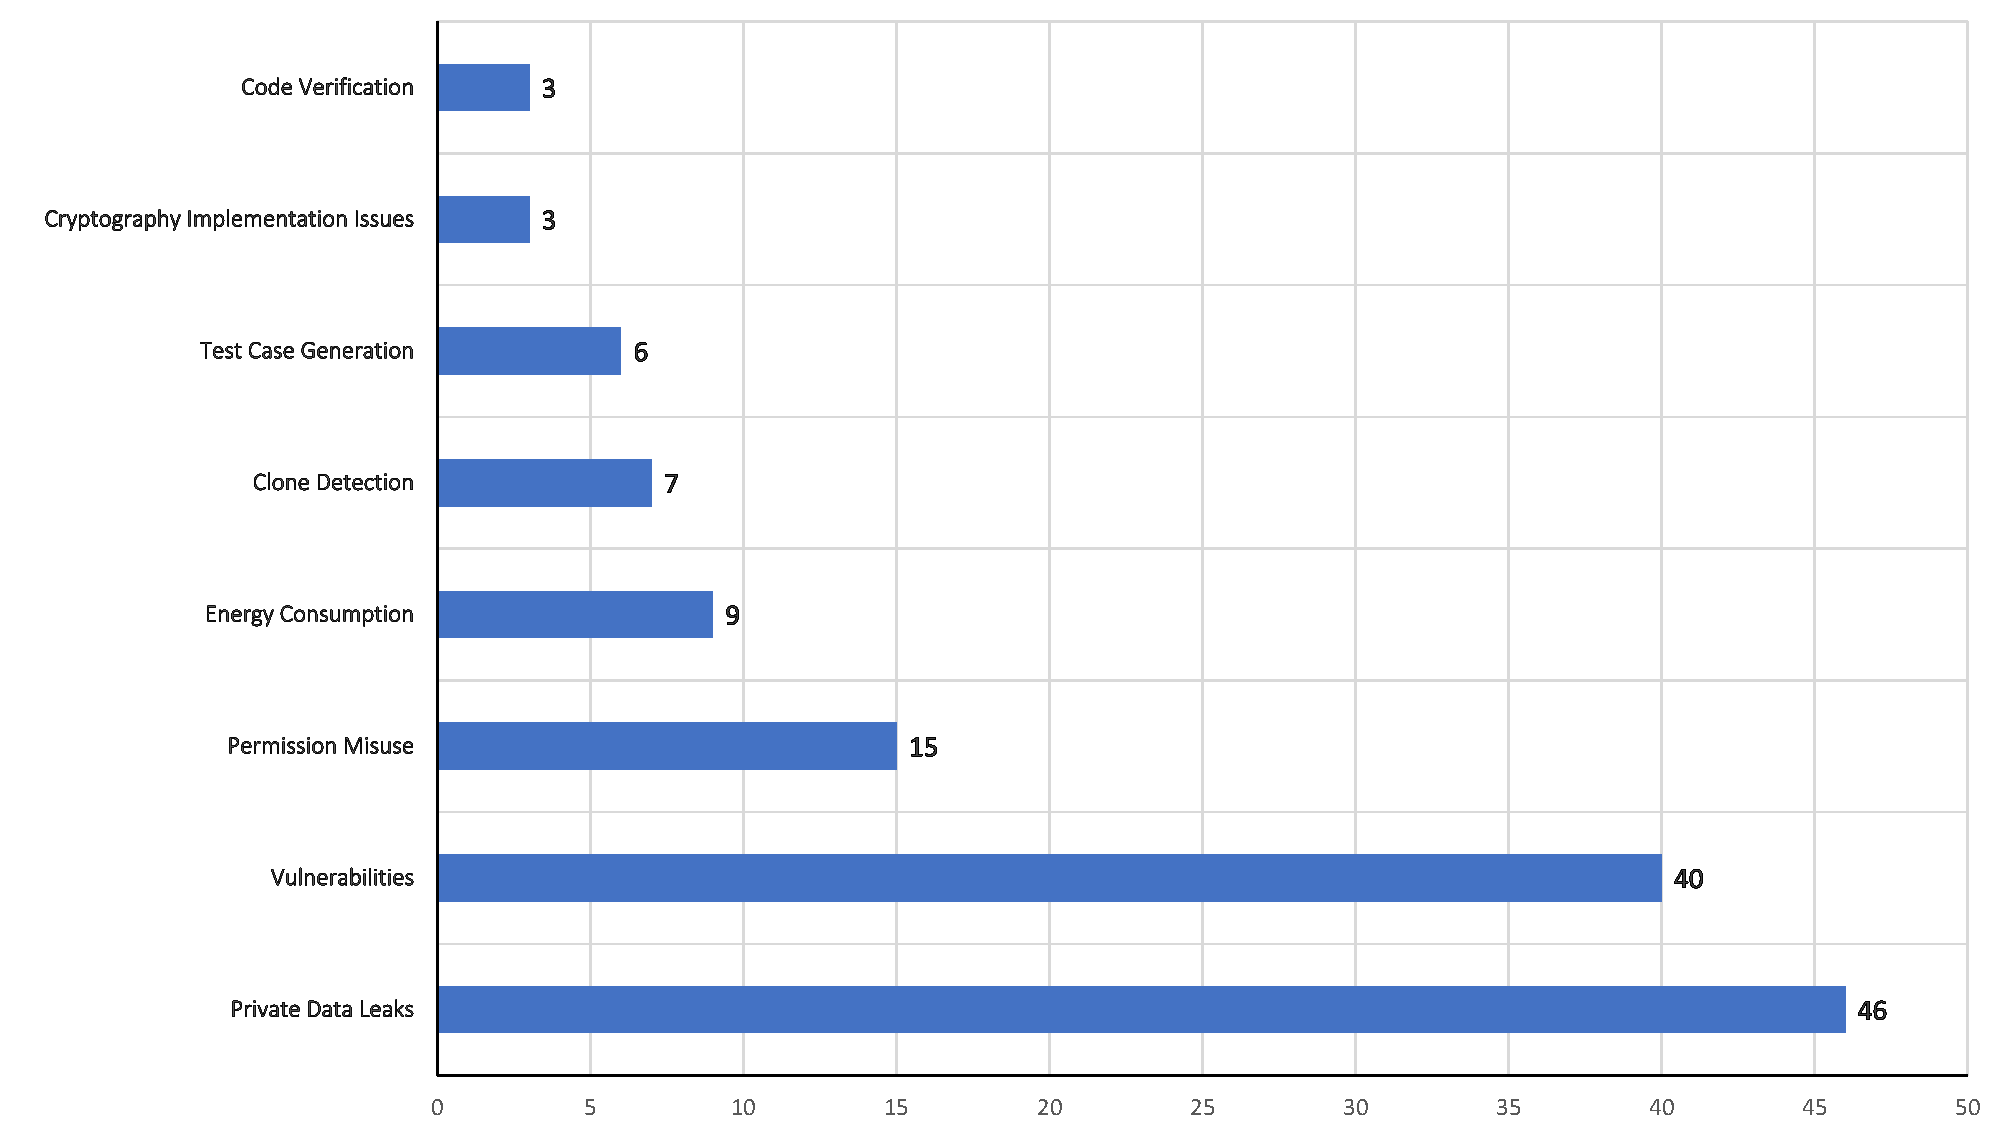
\includegraphics[width=\textwidth]{../Figures/publicationDistribution}
\label{fig:sAPD}
\end{figure}



\textbf{Private Data Leaks.} This is the most frequent purpose reported in the papers categorized by Li \textit{et. al.,}. In this group, FlowDroid is a representative example \cite{Arzt:2014}; FlowDroid  performs static taint analysis on android apps using flow-, context-, field-, object-sensitive and implicit flow-, lifecycle-, static-, alias-aware analysis. Therefore, FlowDroid has became a defacto tool used by researchers interested on finding privacy leaks in Android apps. For example, PCLeaks \cite{li:TrustCom2014} goes one step further by performing sensitive data-flow analysis on top of component vulnerabilities, enabling not only issue identification but also data endangered. The most used intermediate representation for this category of papers is JIMPLE with 18 out of 46 papers, followed by SMALI with 8 papers.

\textbf{Vulnerabilities.} This category groups papers aiming at detecting vulnerabilities in Android apps. For instance,  CHEX\cite{lu:CCS2012} that detects potential component hijacking-based flows through reachability analysis on customized system dependence graphs and, Epicc \cite{octeau:Security2013} and IC3 \cite{octeau:ICSE2015} that implement static analysis techniques for implementing detection scenarios of inter-component vulnerabilities. The most used intermediate representation for this category of papers is SMALI with 15 out of 40 papers, followed by JIMPLE with 6 papers.

\textbf{Permission Misuse.} Permissions are one of the core elements of the Android security model. Malware applications try to use the permissions granted by the user to perform actions that do not correspond to the app features. Lin \textit{et. al.} \cite{lin2014modeling} conducted an study of  permissions that users are most comfortable to grant, creating a set of privacy profiles, and in which way applications use those permissions. The most used intermediate representation for this category of papers is JIMPLE with 6 out of 15 papers, followed by SMALI with 4.

\textbf{Energy Consumption}.  APIs and some hardware components have been demostrated as energy greedy elements in Android apps \cite{Linares-Vasquez:2014,Pathak:2011}, thus, analysis of energy consumption of mobile apps is becoming a hot topic. For instance, Li \textit{et. al.} \cite{li:ISSTA2013} present a tool to calculate source line level energy consumption through combining program analysis and statical modeling. The output of these analyses can then be leveraged to perform quantitative and qualitative empirical investigations into the categories of API calls and usage patterns that exhibit energy consumptions profiles. The most used intermediate representation for this category of papers is JAVA\_CLASS with 6 out of 9 papers, followed by JIMPLE with 2.

\textbf{Clone Detection.} It is also well known that there are some circumstances that lead app users to use APK repositories different from Google Play, which generates a concern about the origin and provenance of Android apps in general. Therefore, approaches such as DNADroid\cite{crussell:ESORICS2012} uses neural networks and dinamic-, static analysis to propose detection of ransomware before infection happens. At the same time, Crusell \textit{et. al.,} \cite{crussell:ESORICS2013} propose a scalable to detecting similar Android Apps based on their semantic information. The most used intermediate representation for this category of papers is SMALI with 3 out of 7 papers, followed by DEX\_ASSEMBLER with 2.

\textbf{Test Case Generation.} A common way to perform analysis of an application is using systematic exploration, nevertheless running real world applications in real devices is cumbersome due to several problems like non-determinism, non-standard control flow, etc. Because of this, A3E\cite{azim:OOPSLA2013} uses static, taint-style, dataflow analysis on the app bytecode to construct a higher level flow-graph that captures legal transition among activities, and can be used to explore the app in a user-like behavior. At the same time, Jensen \textit{et al.}\cite{jensen:ISSTA2013} propose a two-phase technique that uses concolic execution to build summaries of the event handlers of the application and builds event sequences backward from the target, enabling the testing of parts that require more complex event sequences. The most used intermediate representation for this category of papers is JIMPLE with 3 out of 6 papers, followed by WALA\_IR and SMALI with 1 paper each one.

\textbf{Code Verification.} 
Code verification intends to ensure the correctness of a given app but without testing (\textit{i.e.,} app execution). For instance, Cassandra \cite{lortz:SPSMD2014} is proposed to check whether Android apps comply with their personal privacy requirements before installing an app. As another example, researchers have also extended the Julia \cite{payet:IST2012} static analyzer to perform code verification through formal analyses of Android programs. The most used intermediate representation for this category is JAVA\_CLASS with 2 papers.

\textbf{Cryptography Implementation Issues.} In addition to the aforementioned concerns, state-of-the-art works have also targeted cryptography implementation issues. As an example, CMA \cite{shuai2014modelling} performs static analysis on Android apps and select the branches that invoke the cryptographic API. Then it runs the app following the target branch and records the cryptographic API calls. At last, the CMA identifies the cryptographic API misuse vulnerabilities from the records based on the pre-defined model.
It is worth noticing that the top representations used by the reported papers are JIMPLE (38 papers), SMALI (26 papers) and JAVA\_CLASS (22 papers), and the main concern covered is security with around 101 papers.

\begin{figure}[h!]
	\caption{Intermediate representation distribution(i.e., number of papers) vs. purpose of the analysis}
	\centering
	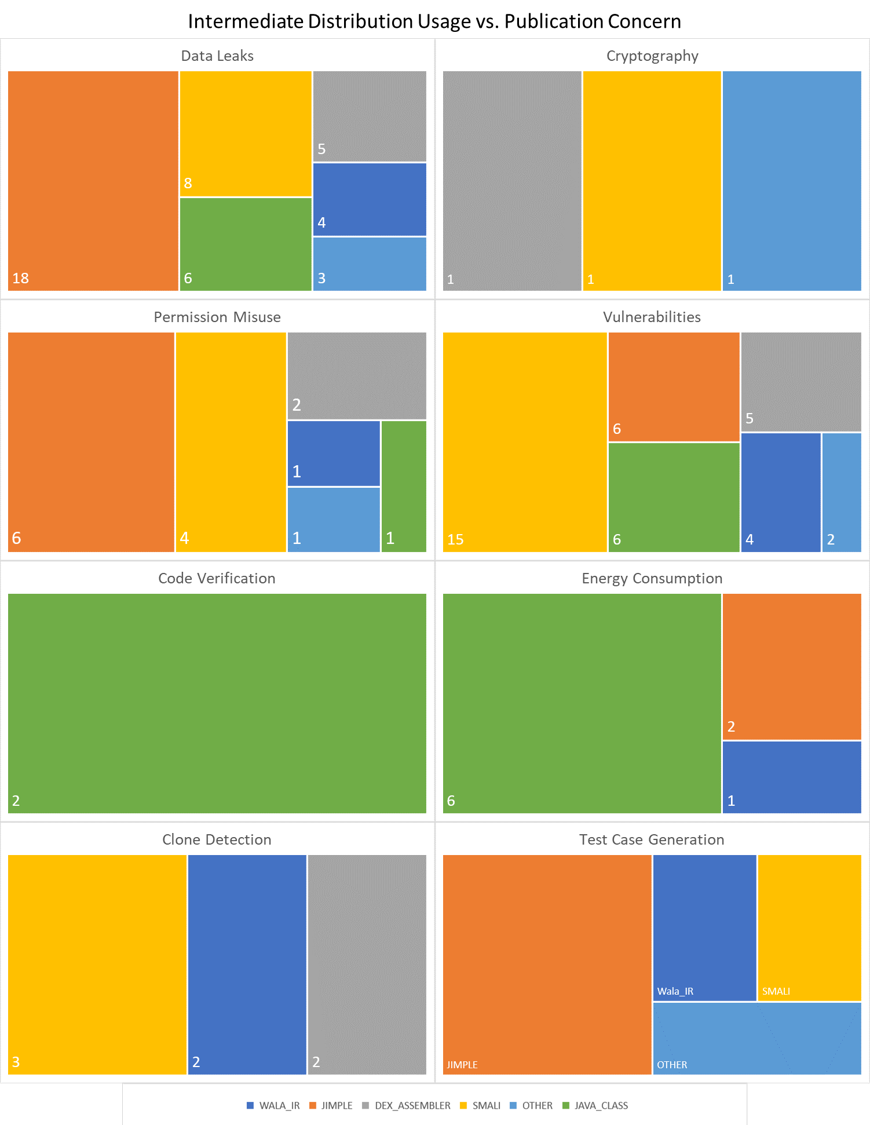
\includegraphics[width=\textwidth]{../Figures/IRvsPC}
	\label{fig:irvspc}
\end{figure}

Therefore, as we wanted to use an intermediate representation that is closer to the compiled code, we have to choose between JIMPLE and SMALI. Because of this, we extended our research to find existing studies aimed at comparing these two intermediate representations. After a short review in google scholar, we found a paper  by Arnatovich \textit{et. al.,}\cite{arnatovich2014empirical} called \textit{Empirical Comparison of Intermediate Representations for Android Applications} in which they study the preserveness of program behavior, by \textit{disassembling, assembling, signing, aligning and installing} 520 applications selected from the Google Play Store. The way they studied this was by running a random GUI-based input generation program (\textit{i.e., monkey runner}) over each app before and after the designed process\footnote{The monkey runner generates a seed that when given as parameter replicates the same events.} and collecting the amount of apps that crashed. Using this result, they were able to identify the amount of apps that do not crash after this process. The results of the study are summarized in Table \ref{tab:cpbp}:

\begin{table}[h!]
	\centering
	\caption{Comparision of program behavior preserveness for SMALI, JIMPLE and JASMIN}
	\label{tab:cpbp}
	\begin{tabular}{|C{3cm}|C{5cm}|}
		\hline
		Intermediate Representation& Preserved Program Behaviors of Original Applications (\%) \\
		\hline \hline
		SMALI&97.68\\
		JIMPLE&85.58\\
		JASMIN&81.92\\
		\hline
	\end{tabular}
\end{table}

Therefore, knowing that SMALI is the intermediate representation that preserves more the program behavior, we decided to use it along with the tool studied to generate mutants that only get affected by the mutation process.

\section{Mutation Testing for Android Apps} \label{sec:MT}

There are some previous work devoted to Mutation testing for Android apps. First, Linares-V\'asquez \textit{et. al.,}\cite{linares2017enabling,Moran:ICSE18} (to the best of our knowledge) have implemented the most comprehensive tool for mutation testing at source code level, MDroid+. They empirically extracted a taxonomy of crashes/bugs in android apps, and based on that, then proposed a set of 38 mutation operators. At the same time, Deng \textit{et al., } \cite{deng2015towards}, presented a set of eight mutant operators oriented to mutate core components of android (\textit{e.g., intents, event handlers, XML files and activity lifecycle}). Deng \textit{et al.} ,presented in 2017 the implementation of their 8 mutation operators in their paper "Mutation Operators for Testing Android Apps"\cite{deng2017mutation}. Finally, the last work found was muDroid\cite{mudroid} a mutation testing tool that works at APK level, but it implements standard mutation operators. However, MDroid+ authors \cite{linares2017enabling,Moran:ICSE18}  found that muDroid generates around 53\% of non-compilable mutants, that can be translated into a lost of half of the time invested on executing muDroid.


% Chapter Template

\chapter{Solution Design} % Main chapter title

\label{ChapterX} % Change X to a consecutive number; for referencing this chapter elsewhere, use \ref{ChapterX}

\section{General Approach} \label{sec:generalApproach}

With the purpose of enabling the execution of software engineering tasks at APK level, we propose a three phase process depicted in Figure \ref{fig:proposeApproach}. The first phase consists of APK processing in order to generate models of the application, and the second phase consists of using those models by a certain module that represent a software engineering task desired by users. The final phase consists in rebuilding the APK when required, as in the case of mutation testing or app instrumentation for dynamic analysis. Note that enabling automated software engineering tasks at APK level is our long term goal, therefore, rebuilding the APK (but whitout decompiling the app to get the source code) is a required step in our approach.

\begin{figure}[htbp]
	\centerline{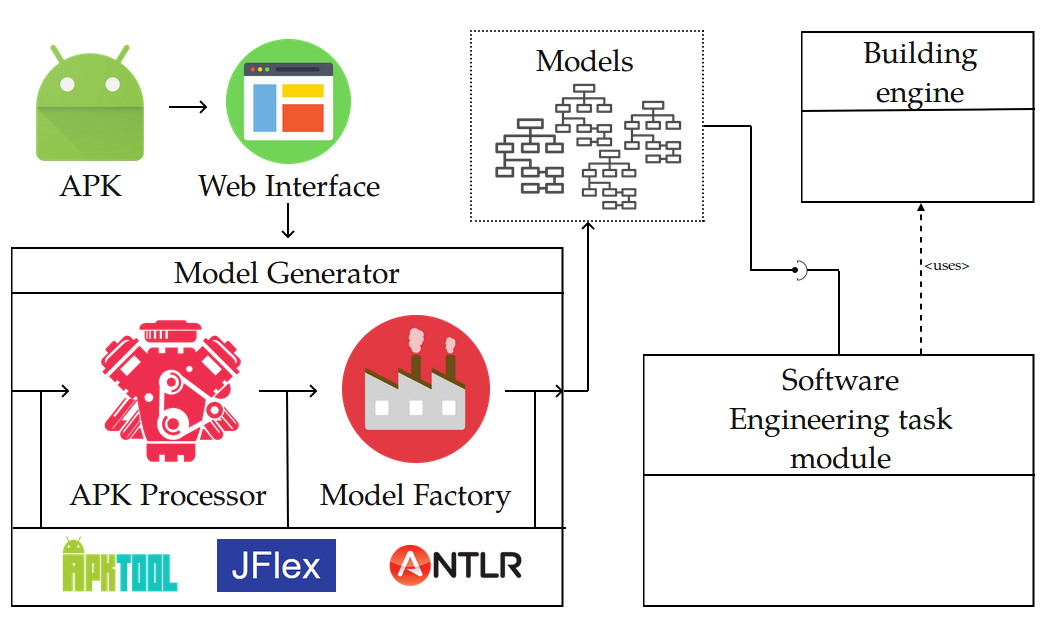
\includegraphics[width=0.9\textwidth]{Figures/proposedApproach.png}}
	\caption{Architecture of the proposed approach}
	\label{fig:proposeApproach}
\end{figure}

\textbf{APK processing.} The first step during the model generation is  decoding an APK file to be able to extract the Android opcodes and resources. Note that an APK is a zip file that contains resources files and a classes file that include the opcodes in DEX format for all the classes belonging to an Android app (including libraries). Based on the wide usage of SMALI as intermediate representation (top 2 according to Li \textit{et. al.,} \cite{li:IST2017}) and that it keeps about 97\% of the information in an APK  \cite{arnatovich2014empirical,arnatovich2018comparison}, we propose it as the representation used for the models extraction. There are already parsers and lexers for SMALI which allows the extraction of abstract syntax trees (ASTs). Concerning the textual information available in resources files, it can be easily extracted because of the XML nature of those files in Android. Note that extracting SMALI code does not require de-compilation to original source code (\textit{e.g.,} Java) which is time consuming and prone to de-compilation errors.

\textbf{Software Engineering Tasks modules.} Because SMALI can be used to extract representations and models such as ASTs, control flow graphs, among others, a plethora of analysis can be instantiated and without the need of original source code. Given the models of the application, implementing a software engineering task must be done on a separate module. These modules must be able to consume the models and provide a comprehensive result to the user. For example, a mutation testing module at APK level must use the AST models extracted from SMALI code to (i) identify the possible mutable snippets of code, and (ii) mutate the original app.


\textbf{Re-building/packaging the app}.
The last phase of this process, consist of going back from decoded SMALI representation to an executable APK file, which does not require recompiling the modified code. However, note that this requires to be very careful when modifying the SMALI code to avoid injecting bugs into the app when the SMALI syntax is not properly used.%For this, we propose to use of APKTool \textit{build} function that from a SMALI representation of an app allows to build an APK. 
This building process must be called by each software engineering task module, making sure all modules that require the execution of this process use the same format to deliver the internal result.



\section{MutAPK}

In order to validate the feasibility of our proposed approach we decided to implement it using mutation testing as a reference. As it was shown in the Section 3, mutation testing is still one of the software engineering tasks that has not been developed at APK level. Consequently, we implemented the proposed approach in a tool ( \textit{\textbf{MutAPK}} ) that allowed us to compare the obtained results when working in the scenarios of having source code, and having only APK files.

As it was mention before, MutAPK must comply to some must-have rules for all mutation testing tools, it has a set of mutant operators, it provides the possibility to select the mutant operators that will be executed, it defines in detail the short process required for its extension and enables parallel execution. MutAPK is an Open Source project available at \url{https://github.com/TheSoftwareDesignLab/MutAPK}. In the following sections, we describe MutAPK according to its workflow described in Figure \ref{fig:mutapkArchitecture}

\begin{figure}[htbp]
	\centerline{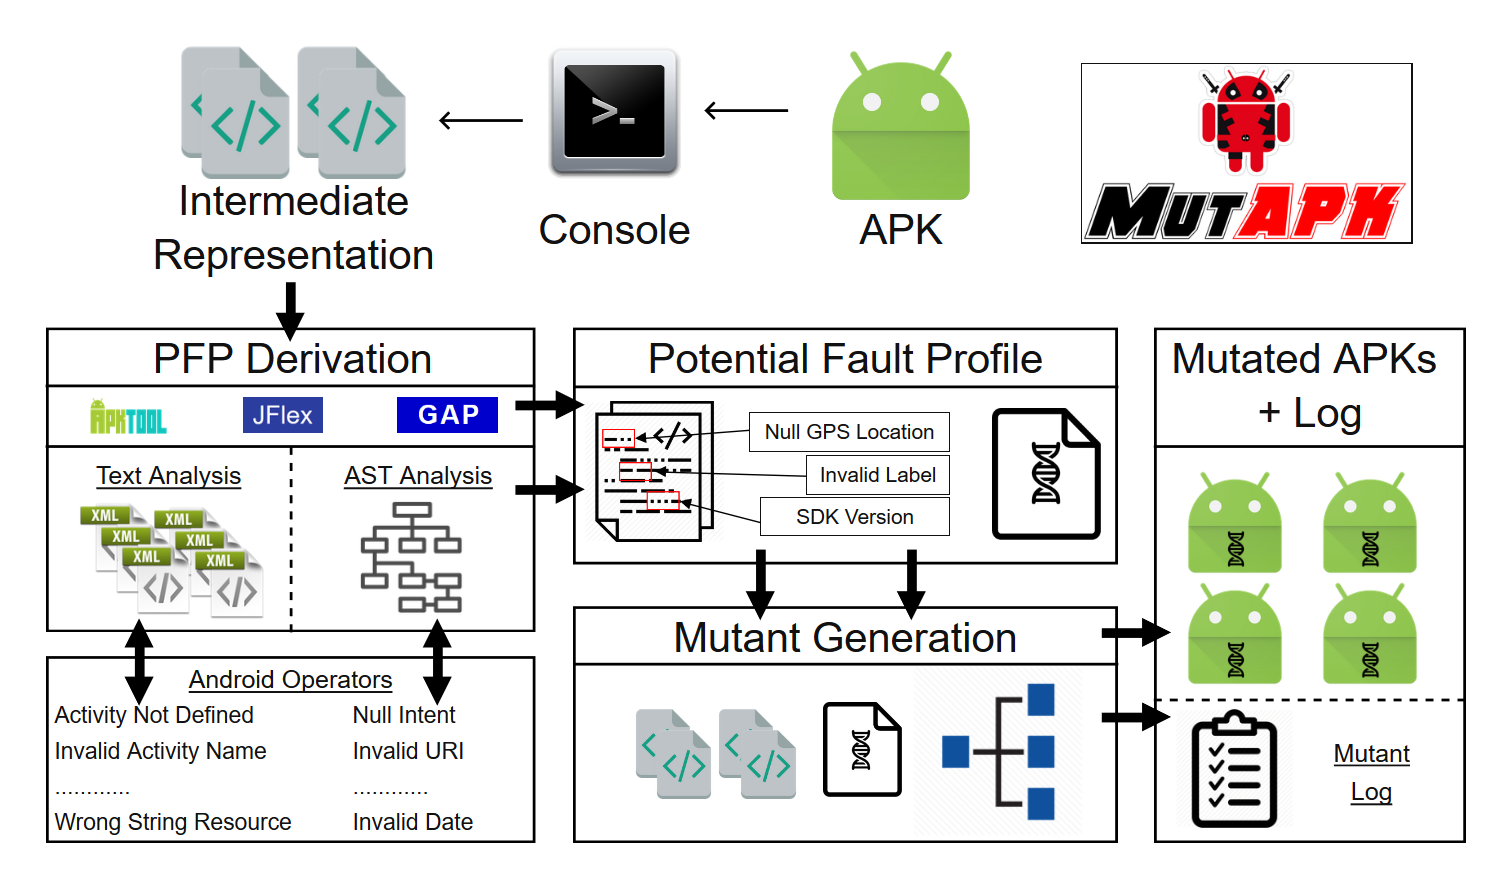
\includegraphics[width=0.9\textwidth]{Figures/mutapkArchitecture.png}}
	\caption{Architecture of MutAPK}
	\label{fig:mutapkArchitecture}
\end{figure}

\subsection{APK Processing}
\subsubsection{Unpackaging/Packaging APK}

Recalling the study by Arnatovich \textit{et al.} \cite{arnatovich2018comparison}, we use APKTool, which allows us to process an APK returning a folder with all the resource files decoded and the source files disassembled into SMALI files. Additionally, code-related files are presented in a useful project like file structure. Because of this, some source code analysis tasks that are based in file location can be easily translated to be executed over APKTool decoding result. At the same time, APKTool allows to build an unsigned apk from the previously mention files. Therefore, an application can be modified in its SMALI representation and then packaged again into an APK for its use.

\subsubsection{Derivation of the Potential Fault Profile}

We followed the same approach proposed by Linares-V\'asquez \emph{et al.} \cite{linares2017enabling,Moran:ICSE18} Therefore, we detect mutation locations by extracting a Potential Fault Profile, and then we implement mutation operations on those locations. The \textit{\textbf{P}otential \textbf{F}ault \textbf{P}rofile \textbf{PFP}} is a set of code locations that represent potential points were a fault can be injected. These potential fault injection points are defined through the mutation operators shown in the Section \ref{sssec:imo}. For the implementation of MutAPK, the PFP definition was inherited from MDroid+. First, both XML and SMALI files are statically analyzed searching for instructions that comply with the characteristics defined in the mutation operators. This previous process, also inherited from MDroid+, consist for XML files of going through the content looking for matches between the file tags and the different mutation operators potential fault injection points. 

On the other hand, for SMALI files the process is based on the Abstract Syntax Tree that is obtained using the lexer and parser created by APKTool to perform the disassembling of an APK. In particular, MutAPK uses the visitor design pattern  to identify the possible locations. Knowing this, the process can easily be extended to add new operators and to provide more comprehensive analysis of the app (\textit{i.e.,} resource and SMALI files) if needed. The final result of the PFP derivation process is a list that joins the potential fault injection points with the mutation operators that can be applied to those locations.
\subsection{Mutation Testing Module}
\subsubsection{Operators}
\label{sssec:imo}
We built upon the 38 operators proposed by  Linares-V\'asquez \emph{et al.} \cite{linares2017enabling,Moran:ICSE18} , which are representative of  potential fault in Android apps and  can be found either on  source code statements, XML tags, or locations in other resource files. In MutAPK we implemented (i) the 33 operators implemented in MDroid+ that do not lead to compilation errors, and (ii) two additional operators not available in MDroid+.

 
Therefore, our work was to translate the  operators implementation from the original source code-based implementations to the corresponding implementations in the SMALI representation. In order to do this, we manually selected 11 apps that had potential locations for implementing the operators. Given those applications, we built the APKs using Android Studio and disassembled manually each one to recognize the direct translation of each mutation original statement. After this dictionary is created, we proceeded to mutate manually the source code of these 11 applications and proceed to generate again the APK files. Finally we performed a diff comparison between the SMALI representation of the original version against the SMALI representation of the mutated version. Because of this, we were able to translate successfully each mutation operator from source code to SMALI representation. With this procedure we derived the list of operators implementation at APK level; the details of each operator are available in our online appendix \cite{MutAPK}.

\subsubsection{Mutant Creation}

We start by unpackaging the apk into a temporal folder. After that, the PFP is derived and a list of potential fault injection locations is created. We now can use the defined mutation rules to generate the mutants, however, in order to make this process as efficiently as possible, MutAPK provides the option to parallelize the mutant creation. For each location in the PFP, a copy of the disassembled apk is created. After the copying ends, based on the mutation operator associated, a new process that translate the mutation rule into an actual change is executed over the exact location inside the associated folder. Next, a compilation process is triggered in order to generate as result an APK. As it was said before, this process can be parallelized and each task consist of: copying the dissambled apk, mutating either a resource file or a SMALI file, and finally compiling the result to obtain an APK.  Nota that while MDroid+ only generates the source code of the mutants, MutAPK is able to generate APKs ready to install and test.

\subsubsection{Extensibility}

Due to the fast change of the android framework, MutAPK must provide the possibility to add new mutation operators easily. Therefore, in order to enable a new mutation operator some changes must be implemented: (i) create a new detector/locator that is capable of finding the correct position that provides all the information needed to create a \textit{Mutation Location} defined in MutAPK; (ii) a mutator, that is capable of using the previously identified location information to mutate the code or resource file; (iii) update the \textit{operator-types.properties} file found under the "src/uniandes/tsdl/mutapk" folder to add the new mutation operator file path with its defined id; (iv) modify \textit{OperatorBundle.java} (in case the new operator is text-based) to add the new text detector and (v) update the \textit{operators.properties} file.

At the same time, MutAPK counts with an \textit{extra} folder where the external libraries are located. Therefore, if user wants to improve the file analysis process or wants to execute a more specialized process over the application, he can save the library files in this folder and manage them easily. MutAPK has in this \textit{extra} folder the \textit{jar} file provided by APKTool. Note that here there is a big difference with MDroid+ implementation; because in MDroid+ the source code must be compiled, then it requires in the extra folder all the libraries required to compile the source, code. This is not required in MutAPK because we are already working with "compiled" code.
\subsection{Tool Usage}
MutAPK has been designed to work as a command line tool. In order to use it, the user must have installed Maven and Java. The MutAPK repository\cite{MutAPK} must be cloned and then packaged using the following commands

\begin{minipage}{\linewidth}
	\begin{lstlisting}[language={sh}, label={lst:mvn}, caption={Git and Maven commands to build MutAPK}, numbers=none]
git clone https://github.com/TheSoftwareDesignLab/MutAPK.git
mvn clean
mvn package
	\end{lstlisting}
\end{minipage}\\

After that, the  jar file called MutAPK-<version>.jar will be located in the \textit{target} folder. That file can be relocated and used in other places. 

\begin{minipage}{\linewidth}
	\begin{lstlisting}[language={sh}, label={lst:ccrM}, caption={Console command to run MutAPK}, numbers=none]
java -jar MutAPK-<version>.jar <APKPath> <AppPackage> <OutputFolder> <ExtraComponentFolder> <operatorsDir> <multithread>
	\end{lstlisting}
\end{minipage}\\

To run it, the previous command must be used (Listing \ref{lst:ccrM}),  where
\begin{enumerate}
	\item \textbf{<APKPath>} is the path to the app's APK
	\item \textbf{<APKPackage>} is the app package used to identify the code that belongs to the app (not the libraries)
	\item \textbf{<OutputFolder>} is the path to the folder where all the mutants will be generated.
	\item \textbf{<ExtraComponentFolder>} is the path to the folder that has the extra libraries used by MutAPK
	\item \textbf{<operatorsDir>} is the path to the \textit{operators.properties} folder, that describes the operators that must be used to generate mutants
	\item \textbf{<multithread>} boolean value, defines if MutAPK must be executed using multiple threads
\end{enumerate}
\begin{minipage}{\textwidth}
	\begin{lstlisting}[language={sh}, label={lst:eompa}, caption={Example Output of MutAPK for PhotoStream app}, numbers=none]
Amount Mutants	Mutation Operator
1		OOM_LARGE_IMAGE
3		NULL_INTENT
5		NULL_OUTPUT_STREAM
1		INVALID_FILE_PATH
5		INVALID_LABEL
19		NULL_VALUE_INTENT_PUT_EXTRA
7		INVALID_COLOR
9		FINDVIEWBYID_RETURNS_NULL
19		INVALID_KEY_INTENT_PUT_EXTRA
5		LENGTHY_GUI_CREATION
8		VIEW_COMPONENT_NOT_VISIBLE
3		NULL_INPUT_STREAM
0		SDK_VERSION
7		INVALID_ACTIVITY_PATH
8		INVALID_VIEW_FOCUS
2		CLOSING_NULL_CURSOR
39		WRONG_STRING_RESOURCE
3		WRONG_MAIN_ACTIVITY
1072		NULL_METHOD_CALL_ARGUMENT
4		NULL_BACKEND_SERVICE_RETURN
2		LENGTHY_GUI_LISTENER
9		INVALID_ID_FINDVIEW
7		ACTIVITY_NOT_DEFINED
5		MISSING_PERMISSION_MANIFEST
2		LENGTHY_BACKEND_SERVICE
3		DIFFERENT_ACTIVITY_INTENT_DEFINITION
Total Locations: 1248
	\end{lstlisting}
\end{minipage}\\

When the command is executed in the console ,  the selected operators and the amount of mutants that are going to be generated for each operator (Listing \ref{lst:eompa}) are logged. Additionally, when all mutants are generated a log of the mutation process can be found at the Output Folder defined in the command. This log allows testers to identify what was the mutation applied on each mutant.

As an extension, for testing purposes MutAPK creates 2 csv files: (i) mutants that were successfully compiled, and (ii) summary of the time consumed to mutate and to compile each mutant. It is worth noting that even if the mutant do not compile correctly the second file register the time it took the compilation to fail.





















%We propose a novel framework aimed at enabling three automated software engineering tasks for Android apps at APK level, i.e., without the need of source code: (i) on-demand developer documentation, (ii) actionable test cases derivation, and (iii) mutants creation for mutation testing. We believe that working with APK files (i) reduces the need of having source code for implementing static analysis approaches that have been proved to be effective, (ii) enables the execution of automated software tasks by third parties that do not access to the source code, and (iii) avoids the overhead introduced by de-compilation process that extracts “original” source code from APKs.
%
%\begin{figure}[htbp]
%\centerline{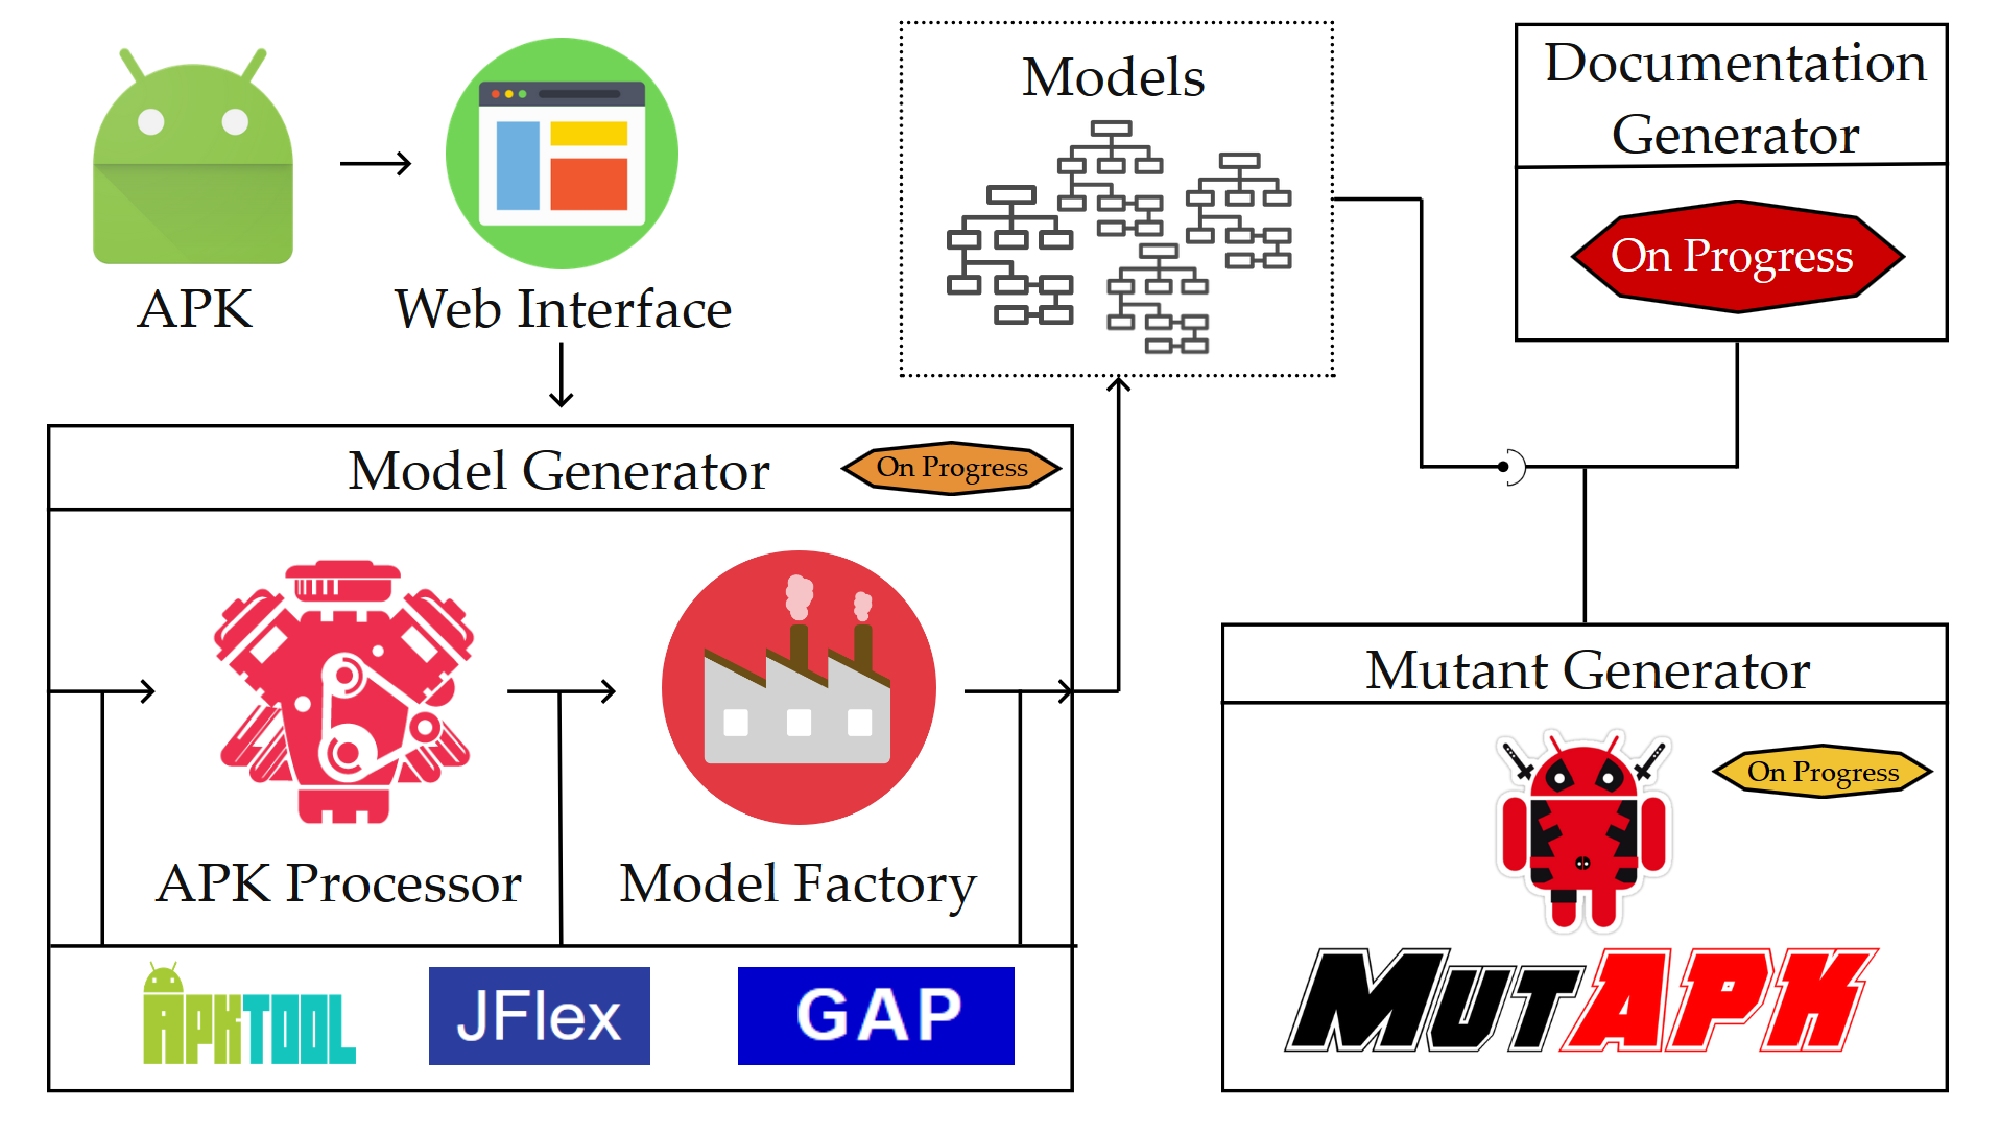
\includegraphics[width=0.9\linewidth]{Figures/Arquitectura}}
%\caption{Proposed Architecture}
%\label{fig}
%\end{figure}
%
%Therefore we present the architecture from the Fig. \ref{fig} that is divide in 4 main sections:
%\subsection*{\textit{\textbf{User Interface}}}
%In order for user to access our tool we present a web interface that will allow to manage the load of an APK, this web interface will be a robust web solution that allows users to: (i) see previous usages of the tool, (ii) access to the models generated for the application and (iii) configure the current usage with the expected results (i.e. on-demand documentation, mutant generation, both of them ).
%
%\subsection*{\textit{\textbf{Model Generator}}}
%Once the user has uploaded the APK the processing task is triggered. This model generator translate the apk into an SMALI representation along with the decoded resources. At this point, it uses a lexer/parser in order to process the SMALI files into a Abstract Sintaxis Tree that will allows the model generator to easily generate other models. At the same time, the model generator process the decoded resources that also provide valuable information as the Android Manifest file, the strings and colors files, creating a representation of the information that can be easily query for further information.
%
%\subsection*{\textit{\textbf{Models storage}}}
%In order to make this tool customizable and extensible we propose that the models generated previously should be stored in a folder where all the extensions tools that enables a software engineering task will search for them. This will allows that other contributors can add other extensions for specific purposes or improve the already created for their needs without worrying of the model generation.
%
%\subsection*{\textit{\textbf{Tool Extensions}}}
%Finally, in order to give real value to the tool, we propose a set of extensions that consumes the models and enables software engineering tasks. For the purpose of this thesis we propose two extensions. The first one is the one in charge of creating documentation for the app. The second one is in charge of creating the mutants for mutation testing.
% Chapter Template

\chapter{Empirical Study} % Main chapter title

\label{ChapterX} % Change X to a consecutive number; for referencing this chapter elsewhere, use \ref{ChapterX}

%----------------------------------------------------------------------------------------
%	SECTION 1
%----------------------------------------------------------------------------------------
\section{Study Design}

The main \textit{goal} of this study is to validate whether the proposed pipeline is feasible, when using a software engineering task as reference and when applied directly to APK files. The \textit{perspective} of the study is of researchers interested in enabling comprehensive solutions for the needed improvement of android app development process. Regarding the \textit{context}, it consist of 54 open source Android applications. In particular, this study aims at answering the following research questions:

\begin{itemize}
	\item \textit{\textbf{$RQ_{1}$}: What is the impact of generating mutants at APK level ?}
	\begin{itemize}
		\item \textit{\textbf{$RQ_{1.1}$}:What is the impact in terms of the amount of generated mutants?}
		\item \textit{\textbf{$RQ_{1.2}$}:What is the impact in terms of the time required to generate a mutant?}
		\item \textit{\textbf{$RQ_{1.3}$}:What is the impact in terms of the amount of compiled mutants?}
		\item \textit{\textbf{$RQ_{1.4}$}:What is the impact in terms of the time required to compile a mutant?}
	\end{itemize}
\end{itemize}

\section{Context of the Study}

In order to present a fair comparison between MutAPK and MDroid+, we have used the same apps MDroid+ used for their experiments. This 54 applications presented in Table \ref{tab:alufs} belong to 16 different categories of the Google Play Store. It is worth noticing that these 54 applications are open source and allows us to study the way code statements are translated from JAVA to SMALI.

In order to collect data that allow us to answer the research question, we compared MutAPK to an existing tool for mutation testing that works at source code level ( MDroid+ \cite{linares2017enabling} ). 
The experiments were executed on a class-server machine. 
Note that in MutAPK, we implemented only 35 of 38 operators listed in Table \ref{tab:cmol} because the other 3 operators lead to non-compilable results. In order to analyze the impact of mutant generation process in MutAPK, we collect: (i) number of mutants generated per mutation operator per application; (ii) number of mutants that compile after mutation; (iii) mutant generation time (\textit{i.e.,} the time required to generate each mutant) and (iv) mutant building times (\textit{i.e.,} the time required to compile each APK file)
\begin{table}[t]
	\centering
	\caption{Applications used for the study}
	\label{tab:alufs}
	\resizebox{0.80\textwidth}{!}{\begin{tabular}{clllc}
			App ID & App Name & Category & Package Name & Version \\
			\hline\hline \\
			1 & A2DP Volume & Transportation & a2dp.Vol & 2.8.11 \\
			2 & AardDictionary & Books \& Reference & aarddict.android & 1.4.1 \\
			3 & FTP Server & Tools & be.ppareit.swiftp\_free & 2.2 \\
			4 & Bites & Lifestyle & caldwell.ben.bites & 1.3 \\
			5 & Battery Circle & Tools & ch.blinkenlights.battery & 1.81 \\
			6 & KeePassDroid & Tools & com.android.keepass & 1.9.8 \\
			7 & LolcatBuilder & Entertainment & com.android.lolcat & 2 \\
			8 & SpriteMethodTest & Sample & com.android.spritemethodtest & 1 \\
			9 & Alarm Clock & Tools & com.angrydoughnuts.android.alarmclock & 1.7 \\
			10 & Translate & Tools & com.beust.android.translate & 1.6 \\
			11 & Quick Settings & Tools & com.bwx.bequick & 1.9.9.4 \\
			12 & Manpages & Productivity & com.chmod0.manpages & 1.51 \\
			13 & BookCatalogue & Productivity & com.eleybourn.bookcatalogue & 3.8 \\
			14 & Mileage & Finance & com.evancharlton.mileage & 3.1.1 \\
			15 & Auto Answer & Tools & com.everysoft.autoanswer & 1.5 \\
			16 & Amazed & Casual & com.example.amazed & 2.0.2 \\
			17 & RandomMusicPlayer & Music & com.example.android.musicplayer & 1 \\
			18 & AnyCut & Productivity & com.example.anycut & 0.5 \\
			19 & HNDroid & News \& Magazines & com.gluegadget.hndroid & 0.2.1 \\
			20 & SpriteText & Sample & com.google.android.opengles.spritetext & - \\
			21 & Triangle & Sample & com.google.android.opengles.triangle & - \\
			22 & Photostream & Media \& Video & com.google.android.photostream & 1.1 \\
			23 & Multi SMS & Communication & com.hectorone.multismssender & 2.3 \\
			24 & World Clock & Tools & com.irahul.worldclock & 0.6 \\
			25 & SyncMyPix & Media \& Video & com.nloko.android.syncmypix & 0.15 \\
			26 & Jamendo & Music & com.teleca.jamendo & 1.0.6-legacy \\
			27 & Yahtzee & Casual & com.tum.yahtzee & 1 \\
			28 & Sanity & Communication & cri.sanity & 2.11 \\
			29 & Mirrored & News \& Magazines & de.homac.Mirrored & 0.2.3 \\
			30 & FileExplorer & Productivity & edu.killerud.fileexplorer & 1 \\
			31 & WeightChart & Health \& Fitness & es.senselesssolutions.gpl.weightchart &	 1.0.4 \\
			32 & SoundBoard & Sample & hiof.enigma.android.soundboard & 1 \\
			33 & ADSdroid & Books \& Reference & hu.vsza.adsdroid & 1.2 \\
			34 & myLock & Tools & i4nc4mp.myLock & 42 \\
			35 & LockPatternGenerator & Tools & in.shick.lockpatterngenerator & 2 \\
			36 & MunchLife & Entertainment & info.bpace.munchlife & 1.4.2 \\
			37 & aGrep & Tools & jp.sblo.pandora.aGrep & 0.2.1 \\
			38 & CountdownTimer & Tools & net.everythingandroid.timer & 1.1.0 \\
			39 & LearnMusicNotes & Puzzle & net.fercanet.LNM & 1.2 \\
			40 & NetCounter & Tools & net.jaqpot.netcounter & 0.14.1 \\
			41 & TippyTipper & Finance & net.mandaria.tippytipper & 1.1.3 \\
			42 & BaterryDog & Tools & net.sf.andbatdog.batterydog & 0.1.1 \\
			43 & Bomber & Casual & org.beide.bomber & 1 \\
			44 & Dialer2 & Productivity & org.dnaq.dialer2 & 2.9 \\
			45 & FrozenBubble & Puzzle & org.jfedor.frozenbubble & 1.12 \\
			46 & aLogCat & Tools & org.jtb.alogcat & 2.6.1 \\
			47 & AnyMemo\_135 & Education & org.liberty.android.fantastischmemo & 8.3.1 \\
			48 & PasswordMakerPro & Tools & org.passwordmaker.android & 1.1.7 \\
			49 & Blokish & Puzzle & org.scoutant.blokish & 2 \\
			50 & ZooBorns & Entertainment & org.smerty.zooborns & 1.4.4 \\
			51 & Wordpress\_394 & Productivity & org.tomdroid & 0.5.0 \\
			52 & MyExpenses & Finance & org.totschnig.myexpenses & 1.6.0 \\
			53 & ImportContacts & Tools & org.waxworlds.edam.importcontacts & 1.1 \\
			54 & Wikipedia & Books \& Reference & org.wikipedia & 1.2.1 \\
		\end{tabular}
	}
\end{table}

\section{Results: Impact of generating mutants at APK level}

\begin{table}[t]
	\centering
	\caption{Comparision at Mutation Operator Level}
	\label{tab:cmol}
	\resizebox{\textwidth}{!}{\begin{tabular}{lC{2cm}lrrrrrrrr}
			&&                      & \multicolumn{2}{c}{\begin{tabular}[c]{@{}c@{}}Amount Mutants\\ Generated\end{tabular}} & \multicolumn{2}{c}{\begin{tabular}[c]{@{}c@{}}Amount Mutants\\ Compiled\end{tabular}}\\
			ID&Mutation Type&Operator Name& MutAPK                                  & MDroid+                                  & MutAPK                                  & MDroid+                                 \\
			\hline \hline \\
			1&Text&ActivityNotDefined&385&384&385&383\\
			2&AST&DifferentActivityIntentDefinition&482&358&120&356\\
			3&Text&InvalidActivityName&383&382&383&382\\
			4&AST&InvalidKeyIntentPutExtra&477&459&62&456\\
			5&Text&InvalidLabel&214&214&214&214\\
			6&AST&NullIntent&482&559&413&556\\
			7&AST&NullValueIntentPutExtra&477&459&452&459\\
			8&Text&WrongMainActivity&56&56&56&56\\
			9&Text&MissingPermissionManifest&227&229&227&229\\
			10&Text&WrongStringResource&3432&3394&3430&3394\\
			11&AST&NotParcelable&0&7&0&1\\
			12&Text&SDKVersion&0&66&0&66\\
			13&AST&LengthyBackEndService&15&8&15&8\\
			14&AST&LongConnectionTimeOut&0&0&0&0\\
			15&AST&BluetoothAdapterAlwaysEnabled&0&4&0&4\\
			16&AST&NullBluetoothAdapter&9&9&9&9\\
			17&AST&InvalidURI&2&2&1&2\\
			18&AST&NullGPSLocation&2&1&2&1\\
			19&AST&InvalidDate&20&40&20&40\\
			20&AST&NullBackEndServiceReturn&34&8&25&7\\
			21&AST&InvalidMethodCallArgument&0&0&0&0\\
			22&AST&NullMethodCallArgument&63441&0&63437&0\\
			23&AST&ClosingNullCursor&222&179&221&166\\
			24&AST&InvalidIndexQueryParameter&82&7&82&6\\
			25&AST&InvalidSQLQuery&82&33&82&33\\
			26&AST&ViewComponentNotVisible&398&347&396&342\\
			27&AST&FindViewByIdReturnsNull&915&413&803&413\\
			28&Text&InvalidColor&47&52&44&52\\
			29&AST&InvalidViewFocus&397&0&393&0\\
			30&AST&BuggyGUIListener&0&122&0&122\\
			31&AST&InvalidIDFindView&915&456&0&452\\
			32&AST&   InvalidFilePath&228&220&226&220\\
			33&AST&NullInputStream&90&61&88&61\\
			34&AST&NotSerializable&0&15&0&8\\
			35&AST&OOMLargeImage&7&7&7&3\\
			36&AST&LengthyGUIListener&339&122&335&122\\
			37&AST&NullOutputStream&59&45&59&45\\
			38&AST&LengthyGUICreation&336&129&330&129\\
			\hline \hline\\
			\multicolumn{3}{c}{\begin{tabular}[c]{@{}c@{}}Total\end{tabular}}&74255&8847&72317&8797\\
	\end{tabular}}
\end{table}

\textbf{\textit{$RQ_{1.1}$}}: To study our results, we present them in two stages, first we show a comparison where only the 33 mutants  in both MDroid+ and MutAPK are taken into account. In Figure \ref{fig:s22agmbp} we show the total amount of generated mutants per app. MutAPK generates around 30 more mutants per app (17\% more than MDroid+). However, if all operators are taken into account, the difference between the amount of mutants get bigger. Figure \ref{fig:agmbp} shows the amount of generated mutants per app. As it can be seen, MutAPK outperforms MDroid+ generating in average 1211 more mutants per app, this corresponds to 7.3 times more mutants. For further analysis of the results at app level, we added the Tables \ref{tab:cal1} and \ref{tab:cal2}, where all info collected is summarized around apps (See Appendix A). Also, we show in Figure \ref{fig:s22agmmobp} that the amount of mutants generated per mutant operator are very similar between MutAPK and MDroid+. It is worth nothing that this figure does not take into account the 63441 mutants generated by one of the operators implemented only in MutAPK. 

\textbf{\textit{$RQ_{1.2}$}}: If we consider again only the 33 shared mutants, in Figure \ref{fig:s22pncmbp} we can see that MutAPK generates around 16\% of non-compilable mutants while MDroid+ generates only 0.5\%. Nevertheless, when using all operators MutAPK generates around 2.36\% of non-compilable mutants while MDroid+ lightly increase its rate to 0.6\%. At the same time, Figure \ref{fig:s22pncmmobp} shows the percentage of non-compilable mutants in terms of the mutant operators, from this we can see that there is also a similar behavior for both. Specifically, MutAPK generates in average 0.1\% non-compilable mutants while MDroid generates 0.05\%.

\textbf{\textit{$RQ_{1.3}$}}: The most important result is the execution time. MutAPK takes only 3\% of the time ( 144,66ms ) required by MDroid+ ( 4,6 seconds) to mutate a copy of the app. Therefore, due to the infraestructure used to run our study, MutAPK takes 9 seconds to generate all mutants for an app (on average), while MDroid takes 19 seconds. 

\textbf{\textit{$RQ_{1.4}$}}: For compilation, MutAPK spends only 6.3\% of the time required by MDroid+ to compile a mutant. Consequently, MutAPK takes 11 min to compile all mutants for an app (on average) while MDroid+ takes 13 min.


Finally, if all mutant operators are selected, MutAPK takes around 9.63 hours to complete the mutation and compilation process for the 54 apps while MDroid+ takes 12 hours.  It is worth remembering that MutAPK generates around 7.3 times more mutants than MDroid+. Therefore, the remaining time could be used by developers,  practitioners, and servers to other software engineering activities. Additionally, as MutAPK generates more mutants, the generated search/bugs space  might be more comprehensive, which means that the quality of the test suite can be tested in a more wide sense.

\begin{landscape}
	\centering
\begin{figure}[t]
	\centering
	\subfigure[\# of Mutants Generated per App without not shared operators]{
		\label{fig:s22agmbp}
		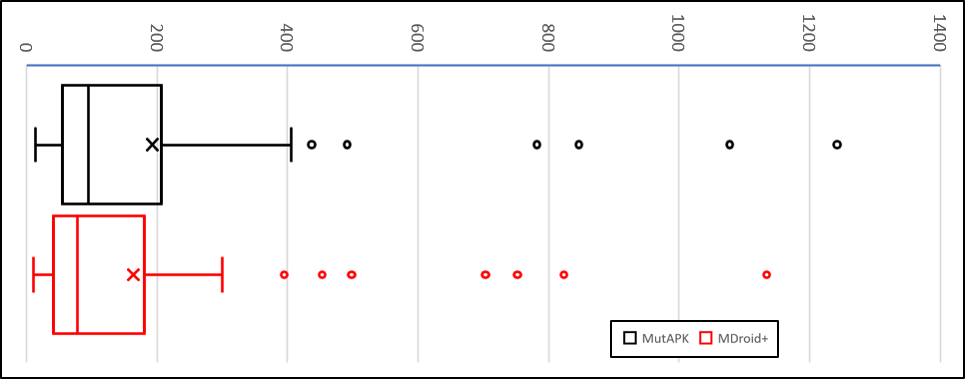
\includegraphics[width=0.35\textheight]{Figures/S22AmountGenMutBP}}
	\subfigure[\% Non-Compilable Mutants without not shared operators]{
		\label{fig:s22pncmbp}
		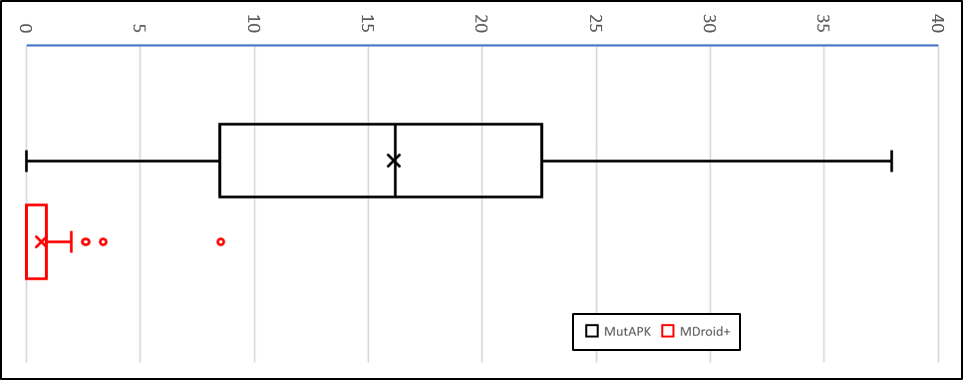
\includegraphics[width=0.35\textheight]{Figures/S22PercNonCompMutBP}}
	\subfigure[\# of Mutants Generated per App]{
		\label{fig:agmbp}
		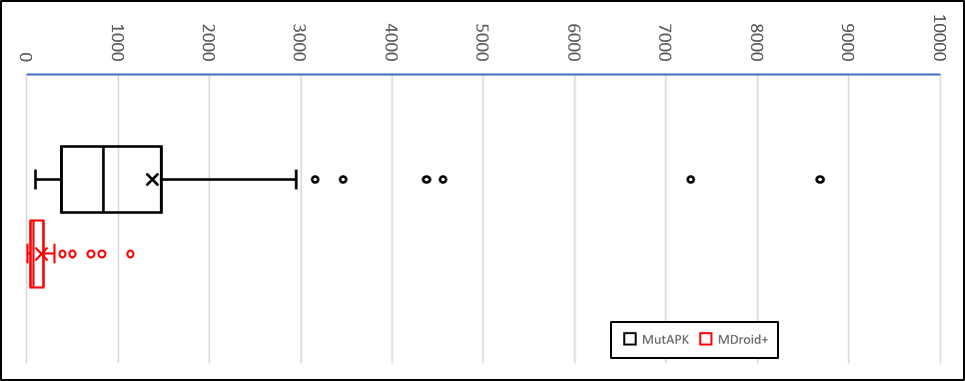
\includegraphics[width=0.35\textheight]{Figures/AmountGenMutBP}}
	\subfigure[\% Non-Compilable Mutants]{
		\label{fig:pncmbp}
		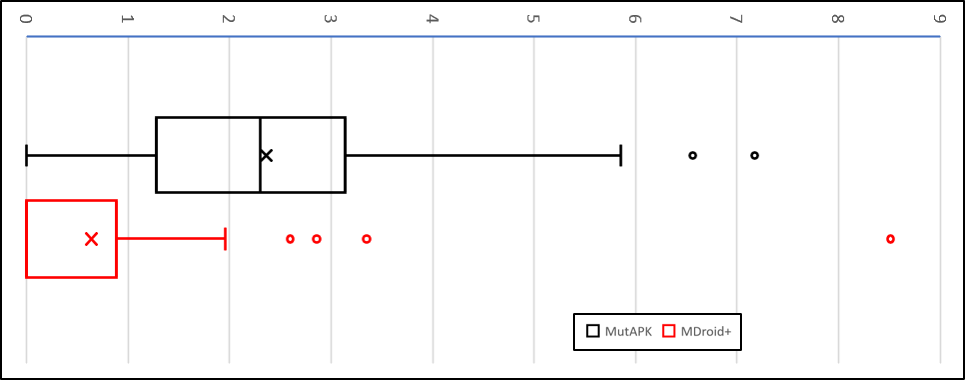
\includegraphics[width=0.35\textheight]{Figures/PercNonCompMutBP}}
	\subfigure[\# of Mutants Generated per mutant operator]{
		\label{fig:s22agmmobp}
		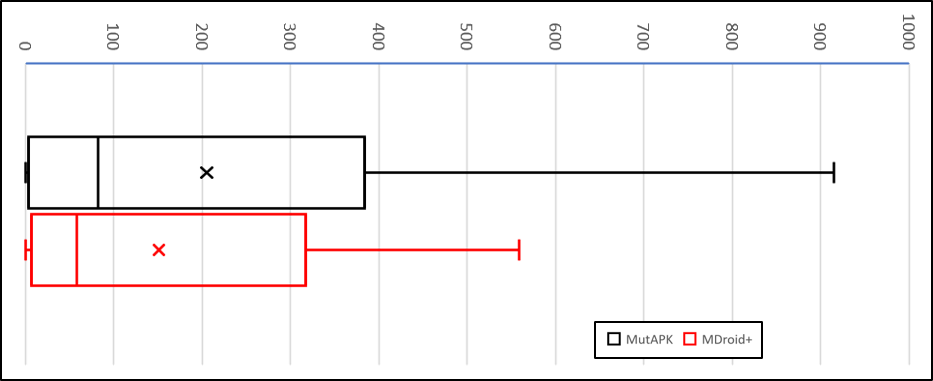
\includegraphics[width=0.35\textheight]{Figures/S22AmountGenMutMOBP}}
	\subfigure[\% Non-Compilable Mutants per mutant operator]{
		\label{fig:s22pncmmobp}
		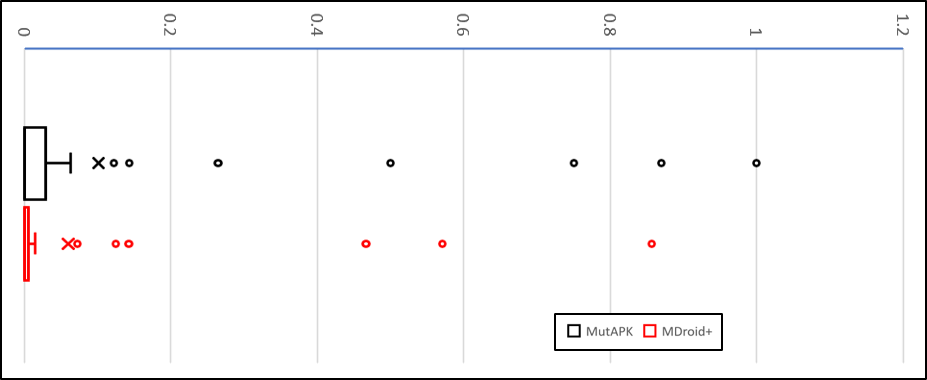
\includegraphics[width=0.35\textheight]{Figures/S22PercNonCompMutMOBP}}
	\caption{Data comparision of MutAPK and MDroid+}
\end{figure}
\end{landscape}

\section{Analysis of non-compilable mutants}

In order to understand the reasons for non-compilable mutants, we analyzed 3 mutants for each one of the mutant operators that generated non-compilable. It is worth noting that this process must be iterative and after finding and fixing the errors, the mutation process must be executed again.

\subsection{31 - InvalidIDFindView}

This operator generated more non-compilable mutants than others. For this operator we found there is an implementation error when the mutation was performed. The correct implementation should be to include \textit{const <constVarName>, 0x<randomlyGeneratedHexa>} before the view was created to assign a random generated value to the key used as view ID. However, we injected \textit{const/16 <constVarName>, 0x<randomlyGeneratedHexa>} that generated a packaging error due to specific instructions that must accompanying \textit{const/16} and not \textit{const}.

After this error was fixed the percentage of non-compilable mutants at app level without taking into account non-shared operators decreases to 4\%.

\subsection{27 - FindViewByIdReturnsNull}

This operator presents two cases we did not consider. Listing \ref{lst:fvbirn1} presents the SMALI representation for finding an Android view; the mutation rule asks to convert the result of the search into a null object. Therefore, Listing \ref{lst:fvbirn2} presents the  SMALI instruction that must be injected instead of the previous one to assign a null value to the result. Nevertheless, after the mutation is performed when the compilation process is launched, an error is displayed on the console (Listing \ref{lst:fvbirn3}), saying that all available registers are between 0 and 15. After a deeper analysis, we found that registers after 16 inclusive are used only for referencing values and a null value could not be assigned. Therefore, we found that a cumbersome process most be made and a verification of the value of the 16th available register must be performed to save the value while the result of the mutation is used, and then the original value can be reassigned to the used register.

This behavior was found in several mutants.

\begin{minipage}{\textwidth}
	\begin{lstlisting}[language={sh}, label={lst:fvbirn1}, caption={SMALI representation of findByViewID method call}, numbers=none]
invoke-virtual {v0, v2}, La2dp/Vol/main;->findViewById(I)Landroid/view/View;

move-result-object v21

check-cast v21, Landroid/widget/Button;
	\end{lstlisting}
\end{minipage}\\

\begin{minipage}{\textwidth}
	\begin{lstlisting}[language={sh}, label={lst:fvbirn2}, caption={SMALI representation of a null value being assigned}, numbers=none]
const/4 v21, 0x0
	\end{lstlisting}
\end{minipage}\\

\begin{minipage}{\textwidth}
	\begin{lstlisting}[language={sh}, label={lst:fvbirn3}, caption={APKTool console response}, numbers=none]
I: Using Apktool 2.3.2
I: Checking whether sources has changed...
I: Smaling smali folder into classes.dex...
test\smali\a2dp\Vol\main.smali[4027,4] Invalid register: v21. Must be between v0 and v15, inclusive.
Could not smali file: a2dp/Vol/main.smali
	\end{lstlisting}
\end{minipage}\\

We found that last line of Listing \ref{lst:fvbirn1} that is in charge of checking the type of the result, is not necessary and can be removed in some cases as it can be seen in Listing \ref{lst:fvbirn4} . Therefore, our implementation search for that instruction to recognize the complete set of instructions that will be replaced. Therefore, MutAPK throws an error when trying to match this expression with next line.

\begin{minipage}{\textwidth}
	\begin{lstlisting}[language={sh}, label={lst:fvbirn4}, caption={APKTool console response}, numbers=none]
invoke-virtual {v7, v9}, Lcom/angrydoughnuts/android/alarmclock/ActivityAlarmNotification;->
	findViewById(I)Landroid/view/View;
	
move-result-object v7
	
invoke-virtual {v7, v12}, Landroid/view/View;->setVisibility(I)V
	\end{lstlisting}
\end{minipage}\\

\subsection{4 - InvalidKeyIntentPutExtra}

Listing \ref{lst:ikipe} shows the result of executing the compilation process over half of the mutants from this mutation operator that are non-compilable. As it can be seen in the listing, the process ends succesfully but no apk file is generated. At this point we think that we might be facing an error within APKTool (\textit{i.e., the tool used for assembling/disassembling an APK}).

\begin{minipage}{\textwidth}
	\begin{lstlisting}[language={sh}, label={lst:ikipe}, caption={Example Output of MutAPK for PhotoStream app}, numbers=none]
I: Using Apktool 2.3.2
I: Checking whether sources has changed...
I: Smaling smali folder into classes.dex...
I: Checking whether resources has changed...
I: Building resources...
S: WARNING: Could not write to (C:\Users\Camilo\AppData\Local\apktool\framework), using C:\Users\Camilo\AppData\Local\Temp\ instead...
S: Please be aware this is a volatile directory and frameworks could go missing, please utilize --frame-path if the default storage directory is unavailable
I: Building apk file...
I: Copying unknown files/dir...
I: Built apk...
	\end{lstlisting}
\end{minipage}\\

If these 4 mutant operators are updated and they do not generate non-compilable mutants, the percentage of non-compilable mutants at APK level (without taking into account the non-shared operators) should be dropped to 0.1\%.






% Chapter Template

\chapter{Conclusion} % Main chapter title

\label{ChapterConclusion} % Change X to a consecutive number; for referencing this chapter elsewhere, use \ref{ChapterX}

We presented in this thesis a novel framework to enable automation of software engineering tasks at APK level through a proposed architecture presented in Section \ref{sec:generalApproach}. Additionally, we validate its feasibility by implementing a Mutation Testing tool called MutAPK \cite{MutAPK}. We evaluate the performance of MutAPK by comparing it with MDroid+, a Mutation Testing tool that works over source code. Our results show that MutAPK outperforms MDroid+ in terms of execution time, generating a testeable APK in a 6.28\% of the time took by MDroid+. In terms of mutant generation MutAPK has a similar behavior to MDroid+ for the shared mutation operators generating about 17\% more mutants (\textit{i.e.,} around 30 more mutants per app). Nevertheless, MutAPK has implemented 2 operators not implemented yet by MDroid+, which enable the generation of about  85\% of the mutants created. Therefore, MutAPK using this operators increases the difference to 739\% more mutants (\textit{i.e.,} around 1211 extra mutants per app).

Nevertheless, the mutation process done by MutAPK needs an improvement due to high rate of non-compilable mutants generated. In average, when using only the shared operators, 16\% of the generated mutants by MutAPK are non-compilable and when all operators are used there are 2.36\%. In this metric, MDroid outperforms MutAPK with only around 0.6\% non-compilable mutants for both cases. Therefore, there is room for improvement because MutAPK should generate only compilable mutants, because it works on already compiled code from source code.

Finally, our results of the initial study with mutation testing suggest that in fact software engineering tasks can be enabled at APK level, and in the particular case of mutation testing we showed that working at APK level improves mutation testing times.
% Chapter Template

\chapter{Future Work} % Main chapter title

\label{ChapterX} % Change X to a consecutive number; for referencing this chapter elsewhere, use \ref{ChapterX}

In this chapter we propose improvements and specialized tasks that could be done after this first stage of the research. First, a more comprehensive search of related work must be done to identify software engineering tasks that has been addressed using static analysis of android apps since 2016. Additionally, this further research can provide more information about the next to be implemented software engineering task (at APK level) in our pipeline, which could be either test cases generation, on-demand documentation, or another one.

At the same time, some effort must be dedicated to fully study the bug taxonomy generated by MDroid+ authors, in order to define more mutation operators or to propose other approaches to identify new possible bugs that could be translated into new mutation operators. Even more important, effort should be devoter to fix the high rate of non-compilable mutants that is generated by MutAPK.

Also, it will be helpful to build a wrapper for MutAPK ( or a new tool ) that is capable of orchestrating the execution of a test suite over the generated mutants. It is important for that solution to offer the possibility of deploying multiple AVD or similar representations and manage them taking into account different challenges as fragmentation, test flakiness, cold starts, etc. \cite{8094439}

As an extension of the research question addressed in this thesis, an extensive study must be done using top applications of the different categories from the Google Play Store, to validate the behavior of MutAPK for more complex applications.
Finally in terms of the implementation of MutAPK, some research effort can be invested in designing a model that improves the location recognition and provides enough information to continue mutating the SMALI representation in the registered times.
%% Chapter Template

\chapter{Implementation} % Main chapter title

\label{ChapterX} % Change X to a consecutive number; for referencing this chapter elsewhere, use \ref{ChapterX}


\section{Activity/Intents}
\subsection{ActivityNotDefined - \textcolor{blue}{Text}}
\begin{lstlisting}[language=XML]
<activity android:name=".ImportActivity" android:label="@string/title_import" />
\end{lstlisting}
 \begin{lstlisting}[language=XML]
 
\end{lstlisting}


\subsection{DifferentActivityIntentDefinition - \textcolor{green}{AST}}
\begin{lstlisting}[language=XML]
Intent intent = new Intent(main.this, ImportActivity.class);
\end{lstlisting}
\begin{lstlisting}[language=XML]
Intent intent = new Intent(main.this, ExportActivity.class); 
\end{lstlisting}
\textcolor{red}{Así se ve en SMALI el código de un Intent}
\begin{lstlisting}[language=XML]
new-instance <intentVar>, Landroid/content/Intent
...
const-class <destClassVar>, L<android:name>
invoke-direct {<intentVar>, <context>, <destClassVar>}
\end{lstlisting}
\subsection{InvalidActivityName - \textcolor{blue}{Text}}
\begin{lstlisting}[language=XML]
<activity android:name=".AboutActivity" android:label="@string/title_about" /> 
\end{lstlisting}

 \begin{lstlisting}[language=XML]
<activity android:name=".AbutActivity" android:label="@string/title_about" /> 
\end{lstlisting}
\subsection{InvalidKeyIntentPutExtra - \textcolor{green}{AST}}
\begin{lstlisting}[language=XML]
intent.putExtra(key, value); 
\end{lstlisting}

\begin{lstlisting}[language=XML]
intent.putExtra("ecab6839856b426fbdae3e6e8c46c38c", value);
\end{lstlisting}

\textcolor{red}{Así se ve en SMALI el código de un Intent}
\begin{lstlisting}[language=XML]
sget-object v5, Lio/github/hidroh/materialistic/OfflineWebActivity;->EXTRA_URL:Ljava/lang/String;
invoke-virtual {v4, v5, p2}, Landroid/content/Intent;->putExtra(Ljava/lang/String;Ljava/lang/String;)Landroid/content/Intent;
\end{lstlisting}
\subsection{InvalidLabel - \textcolor{blue}{Text}}
\begin{lstlisting}[language=XML]
<activity android:name=".VehicleActivity" android:label="@string/title_vehicle" /> 
\end{lstlisting}

\begin{lstlisting}[language=XML]
<activity android:name=".VehicleActivity" android:label="ecab6839856b426fbdae3e6e8c46c38c" /> 
\end{lstlisting}
\subsection{NullIntent - \textcolor{green}{AST}}
\begin{lstlisting}[language=XML]
Intent intent = new Intent(main.this, ImportActivity.class);
\end{lstlisting}

 \begin{lstlisting}[language=XML]
Intent intent = null;
\end{lstlisting}
\subsection{NullValueIntentPutExtra - \textcolor{green}{AST}}
\begin{lstlisting}[language=XML]
intent.putExtra(key, value);
\end{lstlisting}

\begin{lstlisting}[language=XML]
intent.putExtra(key, new Parcelable[0]);
\end{lstlisting}
\subsection{WrongMainActivity - \textcolor{blue}{Text}}
\begin{lstlisting}[language=XML]
<activity android:name=".Mileage" android:theme="@android:style/Theme.NoTitleBar">
	<intent-filter>
		<action android:name="android.intent.action.MAIN" />
		<category android:name="android.intent.category.LAUNCHER" />
	</intent-filter>
</activity> 
\end{lstlisting}

\begin{lstlisting}[language=XML]
<activity android:name=".AboutActivity" android:theme="@android:style/Theme.NoTitleBar">
	<intent-filter>
		<action android:name="android.intent.action.MAIN" />
		<category android:name="android.intent.category.LAUNCHER" />
	</intent-filter>
</activity>
\end{lstlisting}

\section{Android Programming}
\subsection{MissingPermissionManifest - \textcolor{blue}{Text}}
\subsection{NotParcelable - \textcolor{green}{AST}}
\subsection{NullGPSLocation - \textcolor{green}{AST}}
\subsection{SDKVersion - \textcolor{blue}{Text}}
\subsection{WrongStringResource - \textcolor{blue}{Text}}

\section{Back-End Services}
\subsection{NullBackEndServiceReturn - \textcolor{green}{AST}}

\section{Connectivity}
\subsection{BluetoothAdapterAlwaysEnabled - \textcolor{green}{AST}}
\subsection{NullBluetoothAdapter - \textcolor{green}{AST}}

\section{Data}
\subsection{InvalidURI - \textcolor{green}{AST}}

\section{Database}
\subsection{ClosingNullCursor - \textcolor{green}{AST}}
\subsection{InvalidIndexQueryParameter - \textcolor{green}{AST}}
\subsection{InvalidSQLQuery - \textcolor{green}{AST}}

\section{General Programming}
\subsection{InvalidDate - \textcolor{green}{AST}}
\subsection{InvalidMethodCallArgument* - \textcolor{green}{AST}}
\subsection{NotSerializable - \textcolor{green}{AST}}
\subsection{NullMethodCallArgument* - \textcolor{green}{AST}}

\section{GUI}
\subsection{BuggyGUIListener - \textcolor{green}{AST}}
\subsection{FindViewByIdReturnsNull - \textcolor{green}{AST}}
\subsection{InvalidColor - \textcolor{blue}{Text}}
\subsection{InvalidIDFindView - \textcolor{green}{AST}}
\subsection{InvalidViewFocus* - \textcolor{green}{AST}}
\subsection{ViewComponentNotVisible - \textcolor{green}{AST}}

\section{I/O}
\subsection{InvalidFilePath - \textcolor{green}{AST}}
\subsection{NullInputStream - \textcolor{green}{AST}}
\subsection{NullOutputStream - \textcolor{green}{AST}}

\section{Non-Functional Requirements - \textcolor{green}{AST}}
\subsection{LengthyBackEndService - \textcolor{green}{AST}}
\subsection{LengthyGUICreation - \textcolor{green}{AST}}
\subsection{LengthyGUIListener - \textcolor{green}{AST}}
\subsection{LongConnectionTimeOut - \textcolor{green}{AST}}
\subsection{OOMLargeImage - \textcolor{green}{AST}} 
%\include{Chapters/Chapter3}
%\include{Chapters/Chapter4} 
%% Chapter Template

\chapter{Chapter Title Here} % Main chapter title

\label{ChapterX} % Change X to a consecutive number; for referencing this chapter elsewhere, use \ref{ChapterX}

%----------------------------------------------------------------------------------------
%	SECTION 1
%----------------------------------------------------------------------------------------

\section{Main Section 1}

Lorem ipsum dolor sit amet, consectetur adipiscing elit. Aliquam ultricies lacinia euismod. Nam tempus risus in dolor rhoncus in interdum enim tincidunt. Donec vel nunc neque. In condimentum ullamcorper quam non consequat. Fusce sagittis tempor feugiat. Fusce magna erat, molestie eu convallis ut, tempus sed arcu. Quisque molestie, ante a tincidunt ullamcorper, sapien enim dignissim lacus, in semper nibh erat lobortis purus. Integer dapibus ligula ac risus convallis pellentesque.

%-----------------------------------
%	SUBSECTION 1
%-----------------------------------
\subsection{Subsection 1}

Nunc posuere quam at lectus tristique eu ultrices augue venenatis. Vestibulum ante ipsum primis in faucibus orci luctus et ultrices posuere cubilia Curae; Aliquam erat volutpat. Vivamus sodales tortor eget quam adipiscing in vulputate ante ullamcorper. Sed eros ante, lacinia et sollicitudin et, aliquam sit amet augue. In hac habitasse platea dictumst.

%-----------------------------------
%	SUBSECTION 2
%-----------------------------------

\subsection{Subsection 2}
Morbi rutrum odio eget arcu adipiscing sodales. Aenean et purus a est pulvinar pellentesque. Cras in elit neque, quis varius elit. Phasellus fringilla, nibh eu tempus venenatis, dolor elit posuere quam, quis adipiscing urna leo nec orci. Sed nec nulla auctor odio aliquet consequat. Ut nec nulla in ante ullamcorper aliquam at sed dolor. Phasellus fermentum magna in augue gravida cursus. Cras sed pretium lorem. Pellentesque eget ornare odio. Proin accumsan, massa viverra cursus pharetra, ipsum nisi lobortis velit, a malesuada dolor lorem eu neque.

%----------------------------------------------------------------------------------------
%	SECTION 2
%----------------------------------------------------------------------------------------

\section{Main Section 2}

Sed ullamcorper quam eu nisl interdum at interdum enim egestas. Aliquam placerat justo sed lectus lobortis ut porta nisl porttitor. Vestibulum mi dolor, lacinia molestie gravida at, tempus vitae ligula. Donec eget quam sapien, in viverra eros. Donec pellentesque justo a massa fringilla non vestibulum metus vestibulum. Vestibulum in orci quis felis tempor lacinia. Vivamus ornare ultrices facilisis. Ut hendrerit volutpat vulputate. Morbi condimentum venenatis augue, id porta ipsum vulputate in. Curabitur luctus tempus justo. Vestibulum risus lectus, adipiscing nec condimentum quis, condimentum nec nisl. Aliquam dictum sagittis velit sed iaculis. Morbi tristique augue sit amet nulla pulvinar id facilisis ligula mollis. Nam elit libero, tincidunt ut aliquam at, molestie in quam. Aenean rhoncus vehicula hendrerit. 

%----------------------------------------------------------------------------------------
%	THESIS CONTENT - APPENDICES
%----------------------------------------------------------------------------------------

\appendix % Cue to tell LaTeX that the following "chapters" are Appendices

% Include the appendices of the thesis as separate files from the Appendices folder
% Uncomment the lines as you write the Appendices

% Appendix A

\chapter{Detailed Data: Comparison between MutAPK and MDroid+} % Main appendix title

\label{AppendixA} % For referencing this appendix elsewhere, use \ref{AppendixA}

%\section{How do I change the colors of links?}
%
%The color of links can be changed to your liking using:
%
%{\small\verb!\hypersetup{urlcolor=red}!}, or
%
%{\small\verb!\hypersetup{citecolor=green}!}, or
%
%{\small\verb!\hypersetup{allcolor=blue}!}.
%
%\noindent If you want to completely hide the links, you can use:
%
%{\small\verb!\hypersetup{allcolors=.}!}, or even better: 
%
%{\small\verb!\hypersetup{hidelinks}!}.
%
%\noindent If you want to have obvious links in the PDF but not the printed text, use:
%
%{\small\verb!\hypersetup{colorlinks=false}!}.

\begin{landscape}
	\begin{table}[]
		\centering
		\caption{Comparison at Application Level (1)}
		\vspace{-0.3cm}
		\label{tab:cal1}
		\resizebox{0.8\textheight}{!}{
			\begin{tabular}{llrrrrrrrr}
				&                      & \multicolumn{2}{c}{\begin{tabular}[c]{@{}c@{}}Amount Mutants\\ Generated\end{tabular}} & \multicolumn{2}{c}{\begin{tabular}[c]{@{}c@{}}Average Mutation \\Time (ms)\end{tabular}} & \multicolumn{2}{c}{\begin{tabular}[c]{@{}c@{}}Amount Mutants\\ Compiled\end{tabular}} & \multicolumn{2}{c}{\begin{tabular}[c]{@{}c@{}}Average \\ Compilation Time (ms)\end{tabular}}\\
				ID&App Name& MutAPK                                  & MDroid+                                  & MutAPK                                   & MDroid+                                  & MutAPK                                     & MDroid+                                    & MutAPK                                  & MDroid+                                 \\
				\hline \hline\\
				1&A2DPVolume&2862&498&112.92&4611.73&2802&498&14577.16&195320.44\\
				2&AardDictionary&1445&95&1016.18&4611.73&1412&95&54178.4&195320.44\\
				3&FTPServer&1591&88&66.54&4611.73&1590&88&9429.4&195320.44\\
				4&Bites&1378&155&52.19&4611.73&1340&154&7599.57&195320.44\\
				5&Battery Circle&330&44&367.84&4611.73&324&44&10481.15&195320.44\\
				6&KeePassDroid&284&197&450.79&4611.73&282&197&28404.38&195320.44\\
				7&LolcatBuilder&667&55&51.34&4611.73&660&55&6034.63&195320.44\\
				8&SpriteMethodTest&646&42&34.52&4611.73&620&42&6762.62&195320.44\\
				9&AlarmClock&2406&256&113.54&4611.73&2329&254&13109.32&195320.44\\
				10&Translate&651&54&124.25&4611.73&642&54&8048.01&195320.44\\
				11&QuickSettings&2204&395&131.1&4611.73&2139&395&12924.15&195320.44\\
				12&Manpages&384&56&48.32&4611.73&374&55&6054.74&195320.44\\
				13&BookCatalogue&8685&823&433.24&4611.73&8483&816&28977.57&195320.44\\
				14&Mileage&4561&703&391.58&4611.73&4425&701&28005.06&195320.44\\
				15&Auto Answer&202&35&26.24&4611.73&197&35&6107.37&195320.44\\
				16&Amazed&234&10&29.94&4611.73&233&10&5948.88&195320.44\\
				17&RandomMusicPlayer&318&18&54.27&4611.73&315&18&6102.59&195320.44\\
				18&AnyCut&381&77&47.13&4611.73&356&75&5915.5&195320.44\\
				19&HNDroid&1016&123&129.97&4611.73&978&123&16908.1&195320.44\\
				20&SpriteText&894&11&47.54&4611.73&893&11&7137.28&195320.44\\
				21&Triangle&229&11&27.31&4611.73&228&11&5737.86&195320.44\\
				22&Photostream&1236&134&66.7&4611.73&1191&134&8519.48&195320.44\\
				23&MultiSMS&875&102&58.81&4611.73&851&101&6974.07&195320.44\\
				24&WorldClock&2098&65&376.01&4611.73&2071&65&12803.76&195320.44\\
				25&SyncMyPix&2946&244&190.66&4611.73&2902&242&24029.66&195320.44\\
				26&Jamendo&3465&300&272.98&4611.73&3363&295&21041.68&195320.44\\
				27&Yahtzee&423&29&55.94&4611.73&408&29&6382.88&195320.44\\
		\end{tabular}}
	\end{table}
\end{landscape}

\begin{landscape}
	\begin{table}[]
		\centering
		\caption{Comparison at Application Level (2)}
		\vspace{-0.3cm}
		\label{tab:cal2}
		\resizebox{0.8\textheight}{!}{
			\begin{tabular}{llcccccccc}
				&                      & \multicolumn{2}{c}{\begin{tabular}[c]{@{}c@{}}Amount Mutants\\ Generated\end{tabular}} & \multicolumn{2}{c}{\begin{tabular}[c]{@{}c@{}}Average Mutation \\Time (ms)\end{tabular}} & \multicolumn{2}{c}{\begin{tabular}[c]{@{}c@{}}Amount Mutants\\ Compiled\end{tabular}} & \multicolumn{2}{c}{\begin{tabular}[c]{@{}c@{}}Average \\ Compilation Time (ms)\end{tabular}}\\
				ID&App Name& MutAPK                                  & MDroid+                                  & MutAPK                                   & MDroid+                                  & MutAPK                                     & MDroid+                                    & MutAPK                                  & MDroid+                                 \\
				\hline \hline \\
				28&Sanity&4377&752&314.79&4611.73&4315&751&23454.34&195320.44\\
				29&Mirrored&764&98&45.09&4611.73&746&98&6829.19&195320.44\\
				30&FileExplorer&96&13&15.21&4611.73&94&13&4682.15&195320.44\\
				31&WeightChart&1357&209&64.27&4611.73&1314&202&7637.96&195320.44\\
				32&SoundBoard&94&16&21.6&4611.73&92&16&4719.03&195320.44\\
				33&ADSdroid&187&40&165.29&4611.73&183&40&19220.6&195320.44\\
				34&myLock&631&72&45.2&4611.73&615&72&6644.41&195320.44\\
				35&LockPatternGenerator&214&37&36.78&4611.73&210&37&7495.87&195320.44\\
				36&MunchLife&491&57&57.3&4611.73&485&56&6985.63&195320.44\\
				37&aGrep&799&97&51.89&4611.73&774&96&7487.84&195320.44\\
				38&CountdownTimer&565&90&34.08&4611.73&545&90&6332.36&195320.44\\
				39&LearnMusicNotes&473&65&63.13&4611.73&454&65&7632.97&195320.44\\
				40&NetCounter&1558&179&103.57&4611.73&1537&179&12015.31&195320.44\\
				41&TippyTipper&878&55&73.04&4611.73&815&55&7812.34&195320.44\\
				42&BaterryDog&386&23&40.56&4611.73&381&23&6214.73&195320.44\\
				43&Bomber&338&47&32.39&4611.73&338&43&11236.22&195320.44\\
				44&Dialer2&991&186&94.37&4611.73&933&184&7568.09&195320.44\\
				45&FrozenBubble&1030&30&91.27&4611.73&1029&30&9760.92&195320.44\\
				46&aLogCat&702&91&181.65&4611.73&695&91&20487.45&195320.44\\
				47&AnyMemo\_135&7269&1134&617.04&4611.73&6975&1133&32538.12&195320.44\\
				48&PasswordMakerPro&1092&80&161.22&4611.73&1066&79&17459.85&195320.44\\
				49&Blokish&1215&59&71.92&4611.73&1200&59&10696.85&195320.44\\
				50&ZooBorns&508&51&34.31&4611.73&496&50&6778.63&195320.44\\
				51&Wordpress\_394&1437&125&104.28&4611.73&1416&124&12595.55&195320.44\\
				52&MyExpenses&3155&453&135.22&4611.73&3064&447&13738.21&195320.44\\
				53&ImportContacts&997&133&45.28&4611.73&943&133&7351.09&195320.44\\
				54&Wikipedia&241&35&333.31&4611.73&239&34&17303.71&195320.44\\
		\end{tabular}}
	\end{table}
\end{landscape}


%\include{Appendices/AppendixB}
%\include{Appendices/AppendixC}

%----------------------------------------------------------------------------------------
%	BIBLIOGRAPHY
%----------------------------------------------------------------------------------------

\printbibliography[heading=bibintoc]

%----------------------------------------------------------------------------------------

\end{document}  
